%\documentclass[a4paper,]{book}
\documentclass[a4paper, twoside,openright ,titlepage, 12pt]{book}
\usepackage[english]{babel}
\usepackage{preamble}
%\usepackage[MEK,60]{masterfrontpage}
%\setlength\parindent{0pt}


\begin{document}                                                                                                                          
%\maketitle
%\masterfrontpage
\pagenumbering{roman}
\tableofcontents
\newtheorem{theorem}{Theorem}[section]
\newtheorem{lemma}[theorem]{Lemma}
\pagenumbering{arabic}

%\chapter{A motivation for studying fluid-structure interaction}
The interaction between fluid and solids can be observed all around us in nature and has shown crucial in engineering. Examples in nature include swimming fish, flying birds, or trees bending in the wind. Man has learned from nature and has traditionally relied upon laboratory experiments to design windmills, aircrafts, and bridges. The importance of understanding fluid-structure (or solids) interaction (FSI) cannot be overstated, as the lack of such has demonstrated to be disastrous in the design of everything from bridges to airplanes. Let alone to emphasize our incapability to replicate the performance of nature; we're far away from designing a drone capable of flying like a hummingbird. However, laboratory experiments are inherently noisy, expensive, and results can be difficult to reproduce. A much cheaper and indeed smarter approach to studying FSI is using computers, or more specifically numerical simulations to gain fundamental insight to the interaction between fluids and solids. The latter has on the other hand shown to be difficult to realize, for a number of reasons related to both mathematical and computational reasons. Therefore, the goal of this thesis is to develop an open-source framework using standard techniques for solving FSI problems that can be used as a point of reference for future benchmarking of FEniCS-based FSI solvers. \\

The main goal of this thesis is to create a verified and validated monolithic fluid-structure interaction solver in FEniCS, which can handle large deformations. To achieve this, I have defined four subgoals: 

\begin{itemize}
\item Formulate a weak variation for a monolithic arbitrary Lagrangian Eulerian fluid-structure interaction problem.
\item Construct a finite element solver for the fluid-structure interaction problem.
\item Verify and validate a finite element solver for the fluid-structure interaction problem.
\item Compare the impact of discretization and mesh lifting operators on the final solution.
\item Improve computational efficiency of the implementation.
\end{itemize}


Each of the following subgoals will be addressed in separate chapters organized as follows: Balance of linear momentum for both solids and fluids are first introduced together with conservation of mass. The Eulerian, Lagrangian, and the arbitrary Lagrangian-Eulerian (ALE) frames of reference are briefly introduced to express the governing equations, before the equations describing FSI are derived. The numerical implementation is verified using the most rigorous convergence tests, before validation is performed against state-of-the-art benchmarks. Finally, computational speed-up is addressed together with long-term numerical stability of the coupled problem, and methods to overcome these challenges.
 

%\newpage
%\chapter{Governing equations}
%When studying the dynamics of a mediums with fluid or structure %properties under the influence of forces, we need in some sense a good description of how these forces act and alter the system itself.

Computational fluid-structure interaction is a multi-physics field of science, combining two separate fields of computational mechanics, computational fluid dynamics (CFD), and computational structure dynamics (CSM). While CFD and CSM traditionally have been considered as two distinct fields of science,  the goal of CFSI is to combine the separate fluid and structure problems ,and their interaction or \textit{coupling} to one another. Therefore, the study CFSI demands understanding of each separate field. This chapter presents the governing equations of the individual fluid and structure problem, and will form the basis for the next chapter.



\section{Continuum Mechanics}
To interpret nature, mathematical models are needed to describe how object around us reacts to external and/or internal stimuli. 
The mathematical models forms a basis for establishing elementary conservation laws and partial differential equations (PDE's), making scientist and egineers not only able to physical phenomena  in nature, but also predict them. Within mechanics, the response of materials undergoing applied forces or external stimuli is a primary interest. 
Fluid and solids are both materials built up by a sequence of atoms, meaning on a microscopic level, an observer will locate discontinuties and space within the material. Evaluating each atom, or \textit{material point}, is not impossible from a mathematical point of view. However, for mathematical moddeling and applications, the evaluation of each material point remains unpractical. In \textit{Continuum mechanics} (first formulated by Augustin-Louis Cauchy \cite{Merodio2011}), the microscopic structure of materials are  ignored, instead  asuming that the given material of interest is \textit{continously distributed} within the

 A body in continuum mechanics is considered to be matter continuously distributed in space.  Hence, no attention is given to the microscopic (atomic) structure of real materials although non-classical generalized theories of continuum mechanics are able to deal with the mesoscopic structure of matter (i.e. defects, cracks, dispersive lengths, .

To study the influence of forces acting on a continuum, we need an accurate framework to describe the effects. By a continuum we define  to a volume $V(t) \subset \mathbb{R}^d \ d \in (2, 3)$ 
consiting of particles,  continiously distributed throughout its own volume. The initial configuration $V(t = t_0)$  is assumed to be stress free,  defined as the \textit{reference configuration}. A
. We let $V(t)$ for 
$t \geq t_0$ denote the \textit{current configuration}. \\ \\
Central for the coordinate systems introduced in this chapter is the concept of \textit{material} and \textit{spatial} points. \textit{Material} points are simply the points defining the material, moving with it as it undergoes movement. \textit{Spatial} points on the other hand is the relative measure of movement of the \textit{material} points. (Godt nok ??). This concept will be further explained throughout the chapter.

\subsection{The structure problem and agrangian coordinate system}
As some medium is act upon by forces, one of the main properties of interest is the deformation of the medium. Hence we want to know the relative position of some particle from its initial configuration. \\
Let \^{x} be a particle in the reference  $\ha{x} \in \ha{V}$. 
Further let x(\^x, t) be the new location of a particle \^x for some time t such that $x \in V(t)$. We assume that no two particles $\ha{x}_a, \ha{x}_b \in \ha{V}$ occupy the same location for some time $V(t)$.
Then the transformation $\ha{T}(\ha{x}, t) = x(\ha{x}, t)$ maps a particle \ha{x} from the \textit{reference configuration} $\ha{V}$ to the  \textit{current configuration} $V(t)$
Assuming that the path for some \^{x} is continuous in time, we can define the inverse mapping $\ha{T}^{-1}(x, t) = \ha{x}(x, t)$, which maps $x(\ha{x}, t)$ back to its initial location at time $t = t_0$. \\
These mappings lets us track each particle from some \textit{reference configuration} to some deformed state at time t. 
Such a description of tracking each particle $\ha{x} \in \ha{V}$ is often denoted the \textit{Lagrangian Framework} and is a natural choice of describing structure mechanics. 

We define the \textit{deformation} 
\begin{align}
\ha{T}(\ha{x}, t) = \hat{u}(\ha{x},t) = x(\ha{x},t) - \ha{x} 
\end{align}

and the \textit{deformation velocity}
\begin{align}
\pder{\ha{T}(\ha{x}, t)}{t} = \hat{v}(\ha{x},t) = d_t x(\ha{x},t) = d_t \hat{u}(\ha{x},t) 
\end{align}

When tracking each particle as it moves, the \textit{material} and \textit{spatial} points coincide

\subsection{Eulerian coordinate system}
Considering a flow of fluid particles in a river, a \textit{Lagrangian} description of the particles would be tidious as the number of particles entring and leaving the domain quickly rise to a immense number. 
Instead consider defining a view-point $V$ fixed in time, and monitor every fluid particle passing the coordinate $x \in V(t)$ as time elapses. Such a description is defined as the \textit{Eulerian framework.} 
Therefore the Eulerian formulation is natural for describing fluid dynamics. \\
We can describe the particles occupying the \textit{current configuration} $V(t)$ for some time $t \geq t_0$ 
\begin{align*}
x = \ha{x} + \hat{u}(\ha{x}, t)	
\end{align*}
Since our domain is fixed we can define the deformation for a particle 
occupying position $x = x(\ha{x},t)$ as
\begin{align*}
\textbf{u}(x, t) = \hat{u}(\ha{x}, t) = x - \ha{x}	\\
\end{align*}
and its velocity
\begin{align*}
\textbf{v}(x,t) = \partial_t u(x,t) = \partial_t \hat{u}(\ha{x},t) = \hat{v}(\ha{x},t)
\end{align*}

It is important to mention that the we are not interested in which particle is occupying a certain point in our domain, but only its properties. As such the \textit{material} and \textit{spatial} points doesn't coincide in the \textit{Eulerian formulation}


\section{Deformation gradients}
When studying continuum mechanics we observe continious mediums as they are deformed over time. These deformations
results in relative changes of positions due to external and internal forces acting.. These relative changes of postition is called
\textit{strain}, and is the primary property that causes \textit{stress} within a medium of interest \cite{Richter2016}. We define stress as the internal forces that particles within a continuous material exert on each other. \\

The equations of mechanics can be derived with respect to either a deformed or undeformend configuration of our medium of interest. The choice of refering our equations to the current or reference configuration is indifferent from a theoretical point of view. In practice however this choice can have a severe impact on our strategy of solution methods and physical of modelling.   \cite{Wriggers2006}. We will therefore define the strain measures for both configurations of our medium.  

\begin{defn}
Deformation gradient. 
\begin{align}
\hat{F} = I + \hat{\nabla} \hat{u} 
\end{align} 
\end{defn}

Mind that deformation gradient of $\hat{u}$ is which respect to the reference configuration. 
From the assumption that no two particles $\ha{x}_a, \ha{x}_b \in \ha{V}$ occupy the same location for some time $V(t)$, the presented transformation must be linear. As a consequence from the invertible matrix theorem found in linear algebra, the linear operator \textbf{F} cannot be a singuar.  
We define the  \textit{determinant of the deformation gradient} as \textit{J}, which denotes the local change of volume of our domain. 

\begin{defn}
Determinant of the deformation gradient
\begin{align}
J = det(\hat{F}) = det( I + \hat{\nabla} \hat{u} ) \neq 0
\end{align} 
\end{defn}


By the assumption that the medium can't be selfpenetrated, we must limit  J to be greater than 0 \cite{Wriggers2006}

\section{Measures of Strain and Stress}
The equations describing forces on our domain can be derived in accordinance with the current or reference configuration. With this in mind, different measures of strain can be derived with respect to which configuration we are interested in. We will here by \cite{Richter2016} show the most common measures of strain. We will first introduce the right \textit{Cauchy-Green} tensor \textbf{C}, which is one of the most used strain measures \cite{Wriggers2006}. \\ Uttrykk 1.3 fra Godboka, LAG TEGNING \\ 

Let $\ha{x}, \ha{y} \in \ha{V}$ be two points in our referemce configuration and let $\ha{a} = \ha{y} - \ha{x}$ denote the
length of the line bewtween these two points. As our domain undergoes deformation let 
$x = \ha{x} + \hat{u}( \ha{x} ) $ and $x = \ha{y} + \hat{u}( \ha{y} )  $ be the position of our points in the current configuration, and let $a = y - x$ be our new line segment. By \cite{Richter2016} we have by first order Taylor expansion

\begin{align*}
&y - x = \ha{y} + \hat{u}(\ha{y}) - \ha{x} - \hat{u}(\ha{x}) = \
\ha{y} - \ha{x} + \hat{\nabla}\ha{u}(\ha{x}) (\ha{y} - \ha{x}) 
+ \mathcal{O}(|\ha{y} - \ha{x} |^2) \\
&\frac{y - x}{|\ha{y} - \ha{x}|} = [I + \hat{\nabla}\hat{u}(\ha{x} ]  
\frac{\ha{y} - \ha{x}}{|\ha{y} - \ha{x}|} + \mathcal{O}(|\ha{y} - \ha{x} |) 
\end{align*}

This detour from \cite{Richter2016}  we have that 
\begin{align*}
&a = y - x = \hat{F}(\ha{x})\ha{a} +  \mathcal{O}(|\ha{a} |^2) \\
&|a| = \sqrt{ (\hat{F}\ha{a},\hat{F}\ha{a})+ \mathcal{O} (|\ha{a}^3|)  } = 
 \sqrt{ (\ha{a}^T, \hat{F}^T\hat{F}\ha{a})} + \mathcal{O} (|\ha{a}^2|)  
\end{align*}

We let $\ha{C} = \ha{F}^T \ha{F}$ denote the right \textit{Cauchy-Green tensor}.
By observation the Cauchy-Green tensor is not zero at the reference configuration 
\begin{align*}
\ha{C} =  \ha{F}^T \ha{F} = (I + \hat{\nabla} \ha{u})^T (I + \hat{\nabla} \ha{u}) = 1
\end{align*}

Hence it is convenient to introduce a tensor which is zero at the reference configuration. We define the \textit{Grenn-Lagrange strain tensor}, which arises from the squard rate of change of the linesegment \ha{a} and \textit{a}. By using the definition of the Cauchy-Green tensor we have the relation
\begin{align*}
&\frac{1}{2}(|a|^2 + |\ha{a}|^2) = \frac{1}{2}(\ha{a}^T\hat{C}\ha{a}
 -\ha{a}^T \ha{a} ) + \mathcal{O}(|\ha{a}^3| = 
 \ha{a}^T \big(\frac{1}{2} (\hat{F}^T \hat{F} - I) \big) \ha{a} 
 + \mathcal{O}(\ha{a}^3) \\
&\hat{E} = \frac{1}{2}(\hat{C} - I)
\end{align*}

Both the \textit{right Cauchy-Green tensor} $\hat{C}$ and the \textit{Green-Lagrange} $\hat{E}$ are refered to the Lagrangian coordinate system, hence the \textit{reference configuration}. \\
Using similar arguments (see \cite{Richter2016}, compsda) Eulerian counterparts of the Lagrangian stress tensors can be derived.

The \textit{left Cauchy-Green} strain tensor 
\begin{align*}
\mathbf{b} = \ha{F} \ha{F}^T = 
\end{align*}
and the \textit{Euler-Almansi} strain tensor
\begin{align*}
\mathbf{e} = \frac{1}{2} (I - \hat{F}^{-1}\hat{F}^{-T}) = \hat{F}^{-1}\hat{E}\hat{F}^{T}
\end{align*}

It is important to note that strain itself is nothing else than the measurement of line segments under deformation. Therefore strain alone is purely an observation, and it is not dependent on the material of interest. However one expects that a material undergoing strain, will give  forces within the material due to neighboring material interacting with one another. Therefore one derive materialspecific models to describe how a certain material will react to a certain amount of strain.\\
These strain measures are used to define models for \textit{stress}, which is responsible for the deformation in materials (cite holzapfel). The dimention of stress is force per unit area.

\section{Governing Equations}
The fully Fluid-structure interaction problem is based on equations of balance laws, with auxiliary kinematic, dynamic and material relations. In this section, assumptions regarding these relations will be described briefly. A deeper review of the full FSI problem will be considered in the next chapter. 

\subsection{The Fluid}
We will throughout this thesis consider in-compressible fluids described by Navier-Stokes equations. We define the fluid density as $\rho_f$ and fluid viscosity $\nu_f$ to be constant in time. Our phsyical unknowns
fluid velocity $v_f$ and pressure $p_f$ both live in the time-dependent fluid domain  $\hat{\Omega}_f(t)$, with an eulerian configuration. Together with the equations of momentum and continuum, the Navier-Stokes equation is defined as,

\begin{equat}
\textit{Navier-Stokes equation}
\begin{align}
&\rho \pder{\mathbf{v}_f}{t} + \rho \mathbf{v}_f \cdot \nabla \mathbf{v}_f =
\nabla \cdot \sigma + \rho \mathbf{f}_f \hspace{4mm} \text{in} \hspace{2mm} \Omega_f \\
&\nabla \cdot \mathbf{v}_f = 0 \hspace{4mm} \text{in} \hspace{2mm} \Omega_f 
\end{align} 
\end{equat}
where $\mathbf{f}_s$ is some body force. 
Assuming a newtonian fluid the \textit{Cauchy stress sensor} $\sigma$ takes the form \newline $\sigma = -p_f I + \mu_f (\nabla \mathbf{v}_f + (\nabla \mathbf{v}_f)^T$.

Additional appropriate boundary conditions are supplemented to the equation for a given problem. The first type of of boundary conditions are Dirichlet boundary conditions, 
\begin{align}
\mathbf{v}_f = \mathbf{v}_f^D 
\hspace{4mm} \text{on} \hspace{2mm} \Gamma_f^D \subset \partial \Omega_f 
\end{align}
The second type of boundary condition are Neumann boundary conditions
\begin{align}
\sigma_f \cdot \mathbf{n} = \mathbf{g} 
\hspace{4mm} \text{on} \hspace{2mm} \Gamma_f^N \subset \partial \Omega_f 
\end{align}

\newpage
\subsection{The solid}
The governing equations for the solid mechanics are given by the blalance law,
\begin{equat}
\textit{Solid momentum}
\begin{align}
\rho_s \pder{\mathbf{v}_s}{t} = \nabla \cdot \bat{T} + \rho_s \mathbf{f}_s
\hspace{4mm} \text{in} \hspace{2mm} \hat{\Omega}_s
\end{align}
\end{equat}
defined in a Lagrangian coordinate system, with respect to an initial reference configuration $\hat{\Omega}_s$. The structure configuration is given by the displacement $\bat{u}_s$, with the relation
 $\pder{\bat{v}}{t} = \bat{u}_s$ to the solid velocity. The density of the structure is given by $\rho_s$, and $\bat{f}_s$ express any exterior body forces acting. The tensor $\bat{T}$ denotes the first Piola-Kirchhoff stress tensor, with the relation $\bat{T}  = \bat{J} \sigma_s \bat{F}^{-T}$ to the cauchy stress tensor. By definition the cauchy stress tensor is symmetric, however the first Piola-Kirchhoff tensor does not exhibit this property. As constitute equations often assumes this behaviour of symmetry, the second Piola-Kirchhoff tensor $\bat{S}_s$ is convenient as it is symmetric.  It is given by the relation to the firt Piola-Kirchhoff stress tensor by, 
 
 \begin{align*}
 \bat{S}_s = \bat{F}^{-T} \bat{T} = \hat{J} \bat{F}^{-1} \sigma_s \bat{F}^{-T}
 \end{align*}
 
According to the material of interest, several material models exist to model the induced stress given by material deformation. Most famous is Hooke's law, describing a linear relation between strain and stress, limited to a small-deformation regime. As we may no longer be in the range of small-deformation approximation were a linear-elastic material can be used, a consitent way to describe large deformations is needed. As such, for describing large deformation it is widley common to use a stress-strain relation based of the introduced Green Lagrangian strain tensor $\bat{E}$ and the second Piola-Kirchhoff stress tensor $\bat{S}$ \cite{Razzaq2010}. Therefore the material is assumed to follow a hyperelastic model, specifically the Vernant-Kirchhoff(STVK) model. Though STVK can handle large deformations, it is limited of the calculation of large strain \cite{Razzaq2010}. However since the deformations considered in this thesis are small, it will remain our primary choice of strain-stress relation.  STVK describes materials of compressible nature,  but is should be mentioned that for large deformation models describing incompressible materials can be considered. Specially the Incompressible Neo-Hooke (INH) model is considered in several publications (see \cite{Wick2013}, \cite{Richter2010c}), sharing the same hyperelastic properties as the STVK model. As both models handles large deformations, the INH is superior compared to STVK in the sense that it is valid for large strains aswell \cite{Razzaq2010}. \newpage
The STVK is one of the simplest hyperelastic model, as it only extend the famous Hooke's law into a non-linear regime by,

\begin{align*}
\sigma_s = \frac{1}{\hat{J}} \bat{F}(\lambda_s(Tr(\bat{E}) I + 2 \mu \bat{E})\bat{F}^{-T} \hspace{4mm}
\bat{S}_s = \lambda_s(Tr(\bat{E}) I + 2 \mu \bat{E} \\
\bat{E} = \frac{1}{2}(\bat{C} - I ) \hspace{4mm} \bat{C} = \bat{F}\bat{F}^{-T}
\end{align*} 
 where $\bat{C}$ is the right Cauchy-Green strain tensor mention in the last subchapter. 
  
 The solid is often characterized by the Possion ratio and Young modulus. Lamè coefficients  $\lambda_s$ and $\mu_s$ are then given by the relation.

\begin{align*}
&E_y = \frac{ \mu_s ( \lambda_s + 2 \mu_s) }{ ( \lambda_s + \mu_s ) } 
\hspace{5mm} \nu_s = \frac{\lambda_s}{2(\lambda_s + \mu_s)} \\
&\lambda_s = \frac{\nu E_y}{(1 + \nu_s)(1 - 2\nu_s)} \hspace{4mm} \mu_s = \frac{E_y}{2(1 + \nu_s)} 
\end{align*}

Since the solid deformation is a quantity of interest a kinematic condition must be defined for the system of the form
\begin{align}
\pder{\mathbf{v}_s}{t} = \mathbf{u_s} \hspace{4mm} \text{in} \hspace{2mm} \Omega_s
\end{align} 
One might ask the motivation of such an approach as the Lagrangian system could let us define the problem 
\begin{align}
\rho_s \ppder{\mathbf{u}_s}{t} = \nabla \cdot \mathbf{T} + \rho_s \mathbf{f}_s
\hspace{4mm} \text{in} \hspace{2mm} \Omega_s
\end{align}
directly solving for the main quantity of interest namely deformation. However solving for $\mathbf{v}_s$ is more convenient, as it lets us handle constraints for the fluid-structure interaction problem easier. As for the fluid problem we define Dirichlet and Neumann boundary conditions on the form

\begin{align*}
\mathbf{v}_s = \mathbf{v}_s^D 
\hspace{4mm} \text{on} \hspace{2mm} \Gamma_s^D \subset \partial \Omega_s  \\
\sigma_s \cdot \mathbf{n} = \mathbf{g}  
\hspace{4mm} \text{on} \hspace{2mm} \Gamma_s^N \subset \partial \Omega_s 
\end{align*}




%\newpage
%\chapter{Computational Fluid Structure Interaction}

The multi-disciplinary nature of computational fluid-structure interaction , involves addressing issues regarding computational fluid dynamics and computational structure dynamics. In general, CFD and CSM are individually well-studied, in terms of numerical solution strategies. CFSI adds another layer of complexity to the solution process, (1) the \textit{coupling} of the fluid and solid equations , (2) the tracking of \textit{interface} separating the fluid and solid domains. The coupling pose two new conditions at the interface absent from the original fluid and solid conditions, which is \textit{continuity of velocity} and \textit{continuity of stress} at the interface.

\begin{align}
\mathbf{v}_f = \mathbf{v}_s \\
\mathbf{\sigma}_f \cdot \mathbf{n} = \mathbf{\sigma}_s \cdot \mathbf{n}
\end{align}


The tracking of the interface is a issue, due to the different description of motion used in the fluid and solid problem. If the natural coordinate system are used for the fluid problem and solid problem, namely the eulerian and lagrangian description of motion, the domains doesn't match and the interface. Tracking the interface is aslo essential for fulfilling the interface boundary conditions. As such only one of the domains can be described in its natural coordinate system, while the other domain needs to be defined in some transformed coordinate system.   \\ 

Fluid-structure interaction problems are formally divided into the \textit{monolithic} and \textit{partitioned} frameworks.  In the monolithic framework, the fluid and solid equations together with interface conditions are solved simultaneously. The monolithic approach has the advantage of fullfilling the \textit{kinematic} (1.1) and \textit{dynamic}(1.2) interface conditions with high accuracy. The method is then said to be \textit{strongly coupled}. However, the complexity of solving all the equations simuntainiously and the strong coupling contributes to a stronger nonlinear behaviour of the whole system \cite{Wick}. The complexity also makes monolithic implementations \textit{ad hoc} and less modular, and the nonlinearity makes solution time slow.

In the \textit{partitioned} framework one solves the equations of fluid and structure subsequently. Sovling the fluid and solid problems individually is beneficial, in terms of the wide range of optimized solvers and solution strategies developed for each sub-problem. A major drawback is the methods ability to enfore the \textit{kinematic} (1.1) and \textit{dynamic}(1.2) conditions at each timestep. Therefore partitioned solution strategies are defined as  \textit{weakly} coupled. However, by sub-iterations between each sub-problem at each timestep, (1.1) and (1.2) can be enforced with high accuracy, at the cost of increased compuational time. For some applications, low-accuracy of the interface conditions are suffictient such as aeroelasticity \cite{Fernandez2009}. \\

Capturing the interface is matter of its own, regardless of the the monolithic and partitioned frameworks.
The scope of interface methods are divided into \textit{interface-tracking} and \textit{interface-capturing } methods.\cite{Frei2016}. In the \textit{Interface-tracking} method, the mesh moves to accommodate for the movement of the structure as it deformes the spatial domain occupied by the fluid. As such, the mesh itself "tracks" the fluid-structure interface as the domain undergoes deformation. Interface-capturing yields better control of mesh resolution near the interface, which in turn yeilds better control of this critical area in terms of enforcing the interface conditions.
However, moving the mesh-nodes pose potential problems for mesh-entanglements, restricting the possible extent of deformations.  

In \textit{interface-capturing} methods one distinguish the fluid and solid domains by some phase variable over a fixed mesh, not resolved by the mesh iteself. This approach is in general not limitied in terms of deformations, but suffers from reduced accuracy at the interface. \cite{Frei2016}. 

\begin{figure}[h!]
  \centering
    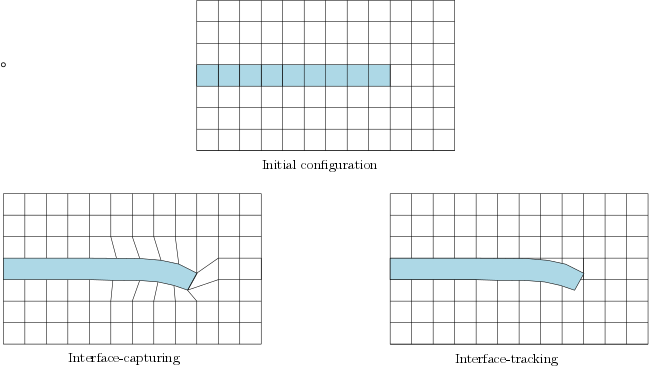
\includegraphics[scale=0.5]{./Fig/interface.png}
      \caption{Comparison of interface-tracking and interface-capturing for an elastic beam undergoing deformation}
\end{figure}

Among the multiple approaches within CFSI, the arbitary Lagrangia-Eulerian methos is chosen for this thesis. 



%We define $\Omega$ in the \textit{reference configuration} be partitioned in a fluid domain $\hat{\Omega_f}$ and a structure domain $\hat{\Omega_s}$ such that
%$\Omega = \hat{\Omega_f} \cup \hat{\Omega_s}$. Further we define the interface $\hat{\Gamma}$ as the interface between these domains such that $\Gamma_i = \hat{\partial \Omega_f} \cap \hat{\partial %\Omega_s}$. 
%The fluid-structure interaction problem is then defined by the fluid and solid equations, and the transmission of the \textit{kinematic} and \textit{dynamic} conditions on the interface $\hat{\Gamma}$. 


%\section{Fully Eulerian}
%This method keeps the fluid in its \textit{Eulerian coordinates}, and such can be seen as the natural counterpart of the ALE method \cite{Wick2013}. First proposed by , \cite{Dunne2006}. One motivation of such and approach is the handling of large-deformation, as the transformation to eulerian coordinates are purely natural.

\section{Arbitary Lagrangian Eulerian formulation}
The \textit{arbitary Lagrangian-Eulerian} formulation is the most popular approach within \textit{Interface-tracking} \cite{Richter2010a}, \cite{Frei2016}, initially developed to combine the strengths of the \textit{Lagranngian} and \textit{Eulerian} coordinate systems. In this approach the structure is given in its natural \textit{Lagrangian coordinate system}, while transforming the fluid domain into an artificial coordinate system similar to the \textit{Lagrangian coordinate system}. Since no natural displacement occur in the fluid domain, the transformation has no directly physical meaning \cite{Richter2010a}, \cite{Donea2004}. 
 
With this in mind, we will derive these transformations with the help of a new arbitary fixed reference system \ha{W}, following the ideas and approaches found in \cite{Richter2016}. Further we denote its deformation gradient as $\hat{F}_w$ and its determinant $\ha{J}_w$. Following the ideas from chapter 2, we introduce the invertibale mapping $\ha{T}_w : \ha{W} \rightarrow V(t)$ , with the scalar $\ha{f}(\ha{x}_W, t) = f(x,t) $ and vector $\hat{w}(\ha{x}_W, t) = \mathbf{w}(x,t) $ counterparts.\\ 
For $\ha{V} = \ha{W}$, $\ha{W}$ simply denotes the familiar Lagrangian description.
In the case $\ha{V} \neq \ha{W}$, $\ha{W}$ as pointed out earlier have no direct physical meaning.  Hence it is important to notice that the physical velocity $\hat{v}$ and the velocity of arbitrary domain $\pder{\ha{W}_w}{t}$ doesn't necessary coincide. This observation is essential, as we will soon see. \\

We will first define the transformation of spatial and temporal derivatives from $V(t)$ to $\ha{W}$ found in \cite{Richter2016}\\

\begin{lem}
Transformation of scalar spatial derivatives \\
\textit{Let f be a scalar function such that} $f: V(t) \rightarrow \mathbb{R}$, \textit{then} 
\begin{align}
\nabla f = \hat{F}_W^{-T} \hat{\nabla}\ha{f}
\end{align} 
\end{lem}

\begin{lem}
Transformation of vector spatial derivatives \\
\textit{Let \textbf{w} be a vector field such that} $\mathbf{w}: V(t) \rightarrow \mathbb{R}^d$, \textit{then} 
\begin{align}
\nabla \mathbf{w} = \hat{\nabla}\hat{w} \hat{F}_W^{-1} 
\end{align} 
\end{lem}

\begin{lem}
Transformation of scalar temporal derivatives \\
\textit{Let f be a scalar function such that} $f: V(t) \rightarrow \mathbb{R}$, \textit{then} 
\begin{align}
\pder{f}{t} = \pder{\ha{f} }{t} - (\hat{F}_W^{-1} \pder{\ha{T}_W}{t} \cdot \hat{\nabla}) \ha{f}
\end{align} 
\end{lem}

In addition we need a consistent way to transform the induced stresses in the \textit{Eulerian} coordinate system to $\ha{W}$. Hence we introduce the \textit{Piloa transformation}, found in most introduction courses in structure mechanics.
\\
\begin{lem}
T \\
\textit{Let \textbf{w} be a vector field such that} $\mathbf{w}: V(t) \rightarrow \mathbb{R}^d$, \textit{then the Piola transformation of w is defined by} 
\begin{align}
\mathbf{w} = \ha{J}_W \hat{F}^{-1}_W \hat{w}
\end{align} 
\end{lem}

The Piola transformation can be further extended to transform tensors, see \cite{Richter2016}, Orange book. This results is essential as it allows us to transform surface forces induced by the \textit{Cauchy stress tensor} on our arbitrary coordinate system $\ha{W}$. Lemma 1.4 brings us to \textit{the first Piola Kirchhoff stress tensor} $\hat{P} = \ha{J}_W \hat{\sigma}\hat{F}_W^{-T}$.

\subsection{ALE formulation of the fluid problem}

Recall the Navier-Stokes equation defined in the \textit{Eulerian coordinate system} V(t).
\begin{align*}
&\rho \pder{\mathbf{v}}{t} + \rho \mathbf{v} \cdot \nabla \mathbf{v} =
\nabla \cdot \sigma + \rho \mathbf{f} \\
&\nabla \cdot \mathbf{v} = 0
\end{align*}
Using our newly introduced transformations of derivatives we map the equation to the arbitrary reference system $\ha{W}$. We will first consider the transformation of the\textit{material derivative}. By 
\begin{align*}
\frac{d \mathbf{v}}{dt}(x,t) = \pder{\mathbf{v}}{t}(x,t) + \nabla \mathbf{v}(x,t) \cdot \pder{x}{t} \\
\frac{d \mathbf{v}}{dt}(x,t) = \pder{\mathbf{v}}{t}(x,t) + \nabla \mathbf{v}(x,t) \cdot \mathbf{v}
\end{align*}
Note $\pder{x}{t}$ is the velocity of particles and not the transformation velocity $\pder{\ha{T}_W}{t}$. By lemma(1.1, 1.2, 1.3) we have  

\begin{align*}
\frac{d \mathbf{v}}{dt}(x,t) = 
\pder{\hat{v}}{t}(x,t) - (\hat{F}_W^{-1}\pder{\ha{T}_W}{t} \cdot \hat{\nabla})\hat{v}
+ \hat{F}_W^{-T}\hat{\nabla}\hat{v} \cdot \hat{v} \\
\mathbf{v} \cdot \nabla \mathbf{v} = \nabla \mathbf{v} \mathbf{v} = 
\hat{\nabla}\hat{v}\hat{F}_W^{-1}\hat{v} = (\hat{F}_W^{-1}\hat{v} \cdot \hat{\nabla})\hat{v} \hspace{4mm} \textit{FINN KILDE}
\end{align*}

These results can be used to show that

\begin{align*}
\pder{\mathbf{v}}{t} + \mathbf{v} \cdot \nabla \mathbf{v} =
\pder{\hat{v}}{t} + (\hat{F}_W^{-1}(\hat{v} - \pder{\ha{T}_W}{t}) \cdot \hat{\nabla}) \hat{v}
\end{align*}

By applying \textit{the first Piola Kirchhoff stress tensor} directly we transform the surface stress by 

\begin{align*}
\nabla \cdot \sigma = \nabla \cdot (\ha{J}_W \hat{\sigma}\hat{F}_W^{-T})
\end{align*}
In general, $\sigma$ is presumed on the form of a Newtonian fluid.
However special care must be taken, as $\sigma \neq \hat{\sigma}$ due to spatial derivatives within the tensor. Hence 
\begin{align*}
\sigma = -p I + \mu_f(\nabla \mathbf{v} + (\nabla \mathbf{v})^T \\
\hat{\sigma} = -\ha{p} I + \mu_f(\hat{\nabla}\hat{v}\hat{F}_W^{-1} +\hat{F}_W^{-T}\hat{\nabla}\hat{v}^T )
\end{align*} 

For the conservation of continuum we apply the \textit{Piola Transformation} such that

\begin{align*}
\nabla \cdot \mathbf{v} = \nabla \cdot (\ha{J} \hat{F}_W^{-1} \hat{v})
\end{align*}

\subsection{ALE formulation of the solid problem}

With the introduced mapping identities we have the necessary tools to derive a full fluid-structure interaction problem defined of a fixed domain. Since the structure already is defined in its natural Lagrangian coordinate system, no further derivations are needed for defining the total problem.

\begin{equat}
\textit{ALE problem on a fixed domain}
\begin{align}
\ha{J} \pder{\hat{v}}{t} + \ha{J} (\hat{F}_W^{-1}(\hat{v} - \pder{\ha{T}_W}{t}) \cdot \hat{\nabla}) \hat{v}
= \nabla \cdot (\ha{J}_W \hat{\sigma}\hat{F}_W^{-T}) + \rho_f \ha{J} \mathbf{f}_f
\hspace{4mm} \text{in} \hspace{2mm} \Omega_f \\
\nabla \cdot (\ha{J} \hat{F}_W^{-1} \hat{v}) \hspace{4mm} \text{in} \hspace{2mm} \Omega_f \\
\rho_s \pder{\hat{v}_s}{t} = \nabla \cdot \mathbf{F}\mathbf{S} + \rho_s \mathbf{f}_s
\hspace{4mm} \text{in} \hspace{2mm} \Omega_s \\
\pder{\hat{v}_s}{t} = \hat{u}_s \hspace{4mm} \text{in} \hspace{2mm} \Omega_s \\
\hat{v}_s = \hat{v}_f \hspace{4mm} \text{on} \hspace{2mm} \Gamma_i \\
\ha{J}_W \hat{\sigma}\hat{F}_W^{-T} \cdot \mathbf{n} = 
\mathbf{F}\mathbf{S} \cdot \mathbf{n}  \hspace{4mm} \text{on} \hspace{2mm} \Gamma_i 
\end{align}
\end{equat}


\subsection*{Fluid mesh movement}
In the ALE framwork one of the most limiting factors is the degeneration of the mesh due to large deformations. Even the most advanced ALE formulated schemes reaches a limit when only re-meshing is nesecarry \cite{Wall12006}. Consequently the choice of an appropriate mesh moving technique is essential to preserve a feasible mesh quality for the simulation of fluid flow. Let the total domain deformation $\ha{T}(\ha{x}, t)$ be divided into the solid and fluid deformation $T_s$, $T_f$, were the fluid deformation is mapped to the arbitrary fixed reference system $\ha{W}$ presented in the last subsection.  
Then the ALE map $T_f$ on the form 
\begin{align*}
\ha{T}_f(\ha{x}, t) = \hat{x} + \hat{u}_f(\hat{x}, t)
\end{align*}
is constructed such that $\hat{u}_f$ is an extension of the solid deformation $\hat{u}_s$ from the interface to the fluid domain. Several extentions have been proposed throuhout the litteratur, and for an overview the reader is refered to \cite{MM2016}, and the reference therein. The construction of such extensions often involves solving some auxiliary problem on a partial differential equation(PDE) form, mainly of second-order. The \textit{Laplacian} and \textit{pseudo-elasticity} extentions are examples, which will be considered in this thesis. These extensions are beneficial in terms of simplicity and computational efficiency, but comes with a cost of user mesh customization. One often want to ensure a desired mesh position and some regularity of mesh spacing on the boundary, but it is impossible for second order extensions to specify both \cite{Helenbrook2003}. Therefore the author of \cite{Helenbrook2003}, proposes a fourth-order PDE, the \textit{biharmonic} extensions, to improve the regularity of the mesh deformation. \\

\subsubsection*{Laplacian model}

The main motivation for a \textit{Laplacian} smoothing is due to its simplicity and due to its property of bounding the interior displacements to the boundary values. 

\begin{align*}
&- \hat{\nabla} \cdot (\alpha^q \hat{\nabla} \hat{u}) = 0 \\
&\hat{u}_f = \hat{u}_s \hspace{2mm} \text{on} \hspace{2mm}  \Gamma \\
&\hat{u}_f = 0 \hspace{2mm} \text{on} \hspace{2mm} \partial \hat{\Omega}_f / \Gamma 
\end{align*}

Most favourable, the largest mesh deformation occuring should be confined to the interal part of the mesh as it causes the least distortion \cite{Jasak2006}. Therefore the introduced diffusion parameter $\alpha$, often raised to some power q, is introduced to manipulate this behaviour. The form of this paramter is often problem specific,  as selective treatment of the elements may vary from different mesh deformation problems. A jacobian based method was introduced in \cite{Stein}. In \cite{Jasak2006}, the authors reviewed several distance based options, where $\alpha$ was some function of the distance to the closest moving boundary. This method was adopted in this thesis on the form

\begin{align*}
\alpha(x) = \frac{1}{x^q}  \hspace{4mm} q = -1
\end{align*}

However as pointed out by \cite{Hsu}, one of the main disadvantages of using the linear Laplace equation is that the equation solves the mesh deformation components independently of one another. Say one have deformation only in the x-coordinate direction, the interior mesh points will only be moved along this deformation. Such a behavior restricts the use to the Laplace equation of mesh extrapolation purposes.

\subsubsection*{Linear elastic model}
Considering a linear elastic model for mesh moving was first introduced in \cite{Tezduyar1992}.  
Both \cite{Dwight}
\begin{align*}
&\nabla \cdot \sigma = 0 \\
&\sigma = \lambda Tr(\epsilon(u)) I + 2 \mu \epsilon(u) \\
&\epsilon(u) = \frac{1}{2}(\nabla u + \nabla  u^T)
\end{align*}

Where Lamé constants $\lambda$ and $\nu$ are given as

\begin{align*}
\lambda = \frac{\nu E}{(1 + \nu)(1 - 2\nu)} \hspace{2mm} \mu = \frac{E}{2(1 + \nu)}
\end{align*}

One of the main motivations for introducing such a model is the manipulation of Young's modulus $E$, and the poisson´s ration $\nu$. Recall that Young's modulus is the measurement of the a materials stiffness, while the poission's ratio describe the materials stretching in the transverse direction under extension in the axial direction. Manipulating these parameters one can influence the mesh deformation,
however the choice of these parameters have proven not to be consistent,  and to be dependent of the given problem.  \\

In \cite{Wicka} the author proposed a negative possion ratio, which makes the model mimic an auxetic material. Such materials becomes thinner in the perpendicular direction when they are submitted to compression, and this property is feasible for mesh under deformation. 

One of the most common approach is to set $\nu$ as a constant in the range $\nu \in [0, 0.5)$ and let $E$ be the inverse of the distance of an interior node to the nearest boundary surface \cite{MM2016}. 
The authors of \cite{Biedron} used this property and also argued that the Young's modulus also could be chosen as the inversely proportional to the cell volume. They also pointed out that both approaches would give the desired result that the small cells around the solid surface would modeled rigid, moving with the surface of the solid as it undergoes deformation. On the other hand cells further away will deform to counter the effects close to the solid surface.

\subsubsection*{Biharmonic model}
Using a biharmonic mesh deformation model provides further freedom in terms of boundary conditions, and the reader is encoured to consult \cite{Helenbrook2003} for a deeper review. We will in combination with \cite{Wicka} present two main approaches the biharmonic model is defined as 
\begin{align*}
\hat{\nabla}^2 \ha{u} = 0 \hspace{4mm} \text{on} \hspace{2mm} \hat{\Omega}_f 
\end{align*}
By introducing a second variable on the form $\ha{w} = - \hat{\nabla} \ha{u}$, we get the following system defined by 
\begin{align*}
&\hat{w} = -\hat{\nabla}^2\hat{u} \\
&- \hat{\nabla} \hat{w} = 0
\end{align*}

This model is defined in a mixed formulation, and as such the prize for quality and control of mesh deformation comes with the cost of more computational demanding problem. 

For the boundary conditions two types has been proposed in \cite{Wicka}. Let 
$\hat{u}_f$ be decomposed by the components $\hat{u}_f = (\ha{u}_f^{(1)}. \ha{u}_f^{(2)})$. Then we have

\begin{align*}
&\textbf{Type 1} \hspace{4mm} \ha{u}_f^{(k)} = \pder{\ha{u}_f^{(k)}}{n} = 0 \hspace{4mm} \partial \hat{\Omega}_f / \Gamma \hspace{2mm} \text{for} \hspace{1mm} k = 1, 2 \\
&\textbf{Type 2} \hspace{4mm} \ha{u}_f^{(1)} = \pder{\ha{u}_f^{(1)}}{n} = 0 
\hspace{2mm} \text{and} \hspace{2mm} \ha{w}_f^{(1)} = \pder{\ha{w}_f^{(1)}}{n} = 0 \hspace{4mm} \text{on} \hspace{1mm} \hat{\Omega}_f^{in} \cup \hat{\Omega}_f^{out} \\ 
&\hspace{17mm}  \ha{u}_f^{(2)} = \pder{\ha{u}_f^{(2)}}{n} = 0 
\hspace{2mm} \text{and} \hspace{2mm} \ha{w}_f^{(2)} = \pder{\ha{w}_f^{(2)}}{n} = 0 \hspace{4mm} \text{on} \hspace{1mm}  \hat{\Omega}_f^{wall}
\end{align*}

With the first type of boundary condition the model can interpreted as the bending of a thin plate, clamped along its boundaries. The form of this problem has been known since 1811, and its derivation has been connected with names like  French scientists Lagrange, Sophie Germain, Navier and Poisson \cite{Meleshko1997}.  

The main motivation for second type of boundary condition is for a rectangular domain where the coordinate axes match the Cartesian coordinate system \cite{Wicka}. In such a configuration, the mesh movement is only constrained in the perpendicular direction of the fluid boundary, leading to mesh movement in the tangential direction. This special case reduces the effect of distortion of the cells.  

\newpage

\newpage
\section{Discretization of the FSI problem}
Say something general of FSI discretization.. FEM, FVM, ...
In this thesis, the finite element method will be used to discretize the coupled fluid-structure interaction problem. It is beyound of scope  of this thesis, to thorough dive into the analysis of the finite element method regarding fluid-structure interaction problems. Only the basics of the method, which is nesecarry in order to define a foundation for problem solving will be introduced. 

\subsection{Finite Element method}
Let the domain $\Omega(t) \subset \mathbb{R}^d \ (d = 1, 2, 3) $  be a time dependent domain discretized a by finite number of d-dimentional simplexes.  Each simplex is denoted as a finite element, and the union of these elements forms a mesh. Further, let the domain be divided by two time dependent subdomains $\Omega_f$ and $\Omega_s$, with the interface $\Gamma = \partial \Omega_f \cap \partial \Omega_s$. The initial configuration $\Omega(t), t = 0 $ is defined as $\hat{\Omega}$, defined in the same manner as the time-dependent domain. $\hat{\Omega}$ is  known as the \textit{reference configuration}, and hat symbol will refer any property or variable to this domain unless specified. The outer boundary is set by $\partial \hat{\Omega}$ , with $\partial \hat{\Omega}^D$ and $\partial \hat{\Omega}^N$ as the Dirichelt and Neumann boundaries respectively. \\ \\

The family of Lagrangian finite elements are chosen, with the function space notation,
\begin{align*}
\hat{V}_{\Omega} := H^1(\Omega) \hspace{4mm} 
\hat{V}_{\Omega}^0 := H_0^1(\Omega)  
\end{align*}
where $H^n$ is the Hilbert space of degree n. \\
Let Problem 2.1 denote the strong formulation. By the introduction of appropiate trial and test spaces of our variables of interest, the weak formulation can be deduced by multiplying the strong form with a test function and taking integration by parts over the domain.  This reduces the differential equation of interest down to a system of linear equations. (skriv bedre..) \\
The velocity variable is continous through the solid and fluid domain
\begin{align*}
\hat{V}_{\Omega, \gat{v}} := \gat{v} \in H_0^1(\Omega), \hspace{2mm} 
\gat{v}_f = \gat{v}_s \ \text{on} \ \hat{\Gamma}_i \\
\hat{V}_{\Omega, \gat{\psi}} := \gat{\psi}^u \in H_0^1(\Omega), \hspace{2mm} 
\gat{v}_f = \gat{v}_s \ \text{on} \ \hat{\Gamma}_i 
\end{align*}
For the deformation, and the artificial deformation in the fluid domain let
\begin{align*}
\hat{V}_{\Omega, \gat{v}} := \gat{u} \in H_0^1(\Omega), \hspace{2mm} 
\gat{u}_f = \gat{u}_s \ \text{on} \ \hat{\Gamma}_i \\
\hat{V}_{\Omega, \gat{\psi}} := \gat{\psi}^v \in H_0^1(\Omega), \hspace{2mm} 
\gat{\psi}_f^v = \gat{\psi}_s^v \ \text{on} \ \hat{\Gamma}_i 
\end{align*}

For simplification of notation the inner product is defined as
\begin{align*}
\int_{\Omega} \gat{v} \ \gat{\psi} \ dx = (\gat{v}, \ \gat{\psi})_{\Omega}
\end{align*}
 

\subsection{Variational Formulation}
With the primaries set, we can finally define the discretization of the monolithic coupled fluid-structure interaction problem. For full transparency, variation formulation of all previous suggested mesh motion models will be shown. For brevity, the laplacian and linear elastic model will be shorted such that 
\begin{align*}
&\hat{\sigma}_{\text{mesh}} = \alpha \nabla \mathbf{u} \hspace{2mm} \text{Laplace} \\
&\hat{\sigma}_{\text{mesh}} =  \lambda Tr(\epsilon(\mathbf{u})) I + 2 \mu \epsilon(\mathbf{u}) \hspace{2mm} \text{Linear Elasticity} 
\end{align*}
Further, only the biharmonic model for the first type of boundary condition will be introduced as the second boundary condition is on a similar form.
  By the concepts of the Finite-element method, the weak variation problem yields.

\begin{prob}
\textit{Coupled fluid structure interaction problem for laplace and elastic mesh moving model.
Find $\bat{u}_s, \bat{u}_f, \bat{v}_s, \bat{v}_f, \ha{p}_f $ such that}
\begin{align*}
\big(\ha{J} \pder{\bat{v}}{t}, \ \gat{\psi}^u \big)_{\hat{\Omega}_f} +
\femf{\ha{J} (\hat{F}_W^{-1}(\bat{v} - \pder{\ha{T}_W}{t}) \cdot \hat{\nabla}) \bat{v}}{\gat{\psi}^u}
+ \femi{\ha{J}_W \hat{\sigma}\hat{F}_W^{-T} \bat{n}_f}{\gat{\psi}^u} \\
- \femf{\ha{J}_W \hat{\sigma}\hat{F}_W^{-T}}{\hat{\nabla}\gat{\psi}^u} -
\femf{\rho_f \ha{J} \mathbf{f}_f}{{\gat{\psi}^u}} = 0 \\
\fems{\rho_s \pder{\bat{v}_s}{t}}{\gat{\psi}^u} + \femi{\bat{F}\bat{S}\bat{n}_f}{\gat{\psi}^u}
- \fems{\bat{F}\bat{S}}{\nabla \gat{\psi}^u} - \fems{\rho_s \bat{f}_s}{\gat{\psi}^u} = 0 \\
\fems{\pder{\bat{v}_s - \bat{u}_s}{t}}{\gat{\psi}^v}  = 0\\
\femf{\nabla \cdot (\ha{J} \hat{F}_W^{-1} \bat{v})}{\gat{\psi}^p} = 0 \\
\femf{\hat{\sigma}_{\text{mesh}}}{\hat{\nabla}\gat{\psi}^u} = 0
\end{align*} 
\end{prob}

\begin{prob}
\textit{Coupled fluid structure interaction problem for biharmonic mesh moving model.
Find $\bat{u}_s, \bat{u}_f, \bat{v}_s, \bat{v}_f, \ha{p}_f $ such that}
\begin{align*}
\big(\ha{J} \pder{\bat{v}}{t}, \ \gat{\psi}^u \big)_{\hat{\Omega}_f} +
\femf{\ha{J} (\hat{F}_W^{-1}(\bat{v} - \pder{\ha{T}_W}{t}) \cdot \hat{\nabla}) \bat{v}}
{\gat{\psi}^u}
+ \femi{\ha{J}_W \hat{\sigma}\hat{F}_W^{-T} \bat{n}_f}{\gat{\psi}^u} \\
- \femf{\ha{J}_W \hat{\sigma}\hat{F}_W^{-T}}{\hat{\nabla}\gat{\psi}^u} -
\femf{\rho_f \ha{J} \mathbf{f}_f}{{\gat{\psi}^u}} = 0 \\
\fems{\rho_s \pder{\bat{v}_s}{t}}{\gat{\psi}^u} + \femi{\bat{F}\bat{S}\bat{n}_f}{\gat{\psi}^u}
- \fems{\bat{F}\bat{S}}{\nabla \gat{\psi}^u} - \fems{\rho_s \bat{f}_s}{\gat{\psi}^u} = 0 \\
\fems{\pder{\bat{v}_s - \bat{u}_s}{t}}{\gat{\psi}^v}  = 0\\
\femf{\nabla \cdot (\ha{J} \hat{F}_W^{-1} \bat{v})}{\gat{\psi}^p} = 0 \\
\femf{\hat{\nabla}\bat{u}}{\hat{\nabla}\gat{\psi}^{\eta}} - 
\femf{\bat{w}}{\hat{\nabla}\gat{\psi}^u} = 0 \\
\femf{\hat{\nabla}\bat{w}}{\hat{\nabla}\gat{\psi}^{v}} = 0
\end{align*}
\text{for the first type of boundary conditions introduced. } 
\end{prob}

Both problems introduced must handle the \textit{kinematic} and \textit{dynamic} boundary conditions in a consistent way. By a continuous velocity field on the whole domain, the \textit{kinematic} condition is strongly enforces on the interface $\hat{\Gamma}_i$
The continuity of normal stresses on the interface are defined as
\begin{align*}
 \femf{\ha{J}_W \hat{\sigma}\hat{F}_W^{-T} \bat{n}_f}{\gat{\psi}^u} = 
  \fems{\bat{F}\bat{S} \bat{n}_s}{\gat{\psi}^u}
\end{align*}
This condition is weakly imposed by omitting the boundary integral from the variational formulation \cite{Wick}, and it becomes an implicit condition for the system. \\


\%newpage
\chapter{Verification and Validation}
 Computer simulations are in many engineering applications a cost-efficient way for conducting design and performance optimalization of physical problems. However, thrusting blindly numbers generated from a computer code can prove to be naive. It doesn't take a lot of coding experience before one realizes the many things that can brake down and produce unwanted or unexpected results. 
Therefore, \textit{credability} of computational results are essential, meaning the simulation is worthy of belief or confidence \cite{Oberkampf2010}. \textit{Verification and validation} (V\&V) is the main approach for assessing and the reliability of computational simulations \cite{Sommerville2006}.  A thorough discussion  of (V\&V) concepts and terminology during the last century can be found in \cite{Oberkampf2010}. In this thesis, the definitions provided by the \textit{American Society of Mechanical Engineers guide for Verification and Validation in Computational Solid Mechanics}  \cite{Schwer2006} are followed.

\begin{defn}
Verification: The process of determining that a computational model accurately represents
the underlying mathematical model and its solution. 
\end{defn}

\begin{defn}
Validation: The process of determining the degree to which a model is an accurate
representation of the real world from the perspective of the intended uses of the model. 
\end{defn}

Simplified \textit{verification} considers if one solves the equations right, while \textit{validation} is checking if one solves the right equations for the given problem \cite{Roache}.

 To test a computational code for all possible parameters, conditions and applications are simply too time consuming.   Verification and validation are therefore ongoing processes, with no clear boundary of completeness unless additional requirements are specified \cite{Roache}. The goal of this chapter is to verify our implementations using the method of manufactured solution  (MMS), addressing validation in a later chapter.

\section{Verification of Code}
Within scientific computing a mathematical model is often the baseline for simulations of a particular problem of interest. For scientists exploring physical phenomena, the mathematical model is often on the form of systems of partial differential equations (PDE´s). A computer program therefore must evaluate  mathematical identities such a differential operators and functions in order to produce accurate solutions of the governing PDE´s. 
Through verification of code, the ultimate goal is to ensure a computer program truly represents the mathematical model. To accumulate sufficient evidence that a mathematical model is solved correctly by a computer code,  it must excel within predefined criteria. If the acceptance criterion is not satisfied, a coding mistake is suspected. Should the code pass the preset criteria, the code is considered verified. Of the different classes of test found in \cite{Roache},  \textit{Order-of-accuracy} (OAA)  is regarded as the most rigorous acceptance criterion for verification \cite{Biggs}, \cite{Roache}, \cite{Etienne2006}. In addition to error estimation and convergence of the numerical solution, the method ensure the discretization error $E$ is reduced in coordinance with the \textit{formal order of accuracy} expected from the numerical scheme. The formal order of accuracy is defined to be the theoretical rate at which the truncation error of a numerical scheme is expected to reduce. The \textit{observed order of accuracy} is the actual rate produced by our code. The order of convergence is calculated  xAssuming a PDE of space and time, order-of-accuracy tests are conducted separatly of 

By monitoring the dicretization error $E$ by spatial and temporal refinements, one assumes the asymptotic behavior,

\begin{align*}
&E = E_x + E_t = u_e - u_h = C\Delta t^p + D\Delta x^l\\
\end{align*} 
where C is a constant, h represents the spatial or temporal resolution, and p is the convergence rate of the numerical scheme. For order of convergence tests, the code is assumed to be verified if the discretization error is proportional to $h^p$.

\subsection{Method of manufactured solution}
The basis of a convergence test is how to find an exact/reference solution, in order to compute the discretization error $E$. However solutions of PDE´s are limited, and often simplifications of the original problem are needed to produce analytically solutions.  \textit{The method of manufactured solutions} provides a simple yet robust way of making analytic solutions for PDE´s. 
Let a  partial differential equation of interest be on the form
\begin{align*}
\textbf{L}(\textbf{u}) = \textbf{f}
\end{align*}

Here \textbf{L} is a differential operator, \textbf{u} is variable the of interest, and \textbf{f} is some sourceterm. In the method of manufactured solution one first manufactures a solution \textbf{u} for the given problem. In general, the choice of \textbf{u} will not satisfy the governing equations, producing a sourceterm  \textbf{f} after differentiation by \textbf{L}. The produced source term will cancel any imbalance formed by the manufactured solution \textbf{u} of the original problem. Therefore, the manufactured solution can be constructed without any physical reasoning, proving code verificaion as a purely a mathematical exercise were our only interest is to verify the solution \cite{Roache2002}. If the MMS is not chosen properly the test will not work, therfore some guidelines for rigirous verification have been proposed in \cite{Etienne2006, Biggs, Roache2002}. 

\begin{itemize}
\item The manufactured solution (MS), should be composed of smooth analytic functions such as exponential, trigonometric, or polynomials.
\item The MS should should have sufficient number of derivatives, exercising all terms and derivatives of the PDE´s. 
\end{itemize}

To deeply verify the robustness of the method of manufactured solution,  a report regarding code verification by MMS for CFD was published by Salari and Knupp \cite{Biggs}. This thorough work applied the method for both compressible and incompressible time-dependent Navier-Stokes equation. To prove its robustness the authors deliberate implemented  code errors in a verified Navier-Stokes solver by MMS presented in the report. In total 21 blind testcases where implemented, where different approaches of verification frameworks were tested. 
Of these, 10 coding mistakes that reduces the observed order-of-accuracy was implemented. Here the method of manufactured solution captured all coding mistakes, except one. This mistake would, accordingly to the co-author , been captured if his guidelines for conducting MMS had been followed. 
In general, computing the source term f can be quite challenging and error prone.  Therefore, symbolic computation of the sourcterm is advantigous to overcome mistakes which can easily occur when calulating by hand. For construction of the sourceterm \textbf{f}, the Unified Form Language (UFL) \cite{Alnes2015} provided in FEniCS Project will be used. 

\subsection{Verification of the fluid-structure interaction solver by MMS}
In general the MMS does not need to match any physical capabilities. However, when considering multiphysics problems, such as FSI, the equations has to meet the mathematical criteria of the interface.
\begin{enumerate}
\item Kinematic boundary condition $\bat{v}_s = \bat{v}_f$, enforced strongly by a continious velocity field in the fluid
        and solid domain.
\item Dynamic boundary condition $\sigma_s \cdot \mathbf{n}= \sigma_f \cdot \mathbf{n}$, enforced weakly by omitting the 
        boundary integrals from the weak formulation in problem.
\end{enumerate}
The choice of a MMS is therefore not trivial, as it must fulfill condition 1 and 2, in addition to the divergence-free condition in the fluid, and avoiding cancellation of the ALE-convective term $/pder{\hat{T}_f}{t}$.  The struggle is reflected of the abscence of research, regarding MMS for coupled FSI solvers in the litterature. The challenge are often disregarded, such as \cite{Sheldon2014}, where the verification process is conducted on the fluid and structure solver separately. Instead, the correctness of the coupling is evaluated by the code validation. The approach clearly ease the process, assuming verification of each codeblock is "sufficient" to declare the code verified. It must be stressed that solving each problem individually is not true verification, in reference to a monolithic approach where the problems are solved at the same time.\\The construction of a MMS for a monolithic FSI problem is therefore out of the scope of this thesis. Conducting verification on the fluid and structure separatly is not , but considered "good enough" to show the mathematical model is discretized accuratly.

\section{Validation}
Through \textit{verification}, one can assure that a scientific code implements a mathematical model correctly. However, correctness is unnecessary if the model fails to serve as an accurate representation of the physical problem of interest. 
By definition 1.2, \textit{Validation} is the act of demonstrating that a mathematical model is applicable for its intended use with a certain degree of accuracy. That is, a mathematical model is validated if it meets some predefined criteria within a specific context. Validation is therefore not intended to portray the model as an absolute truth, nor the best model available \cite{Rykiel1996}. In computational science, validation is conducted by comparing numerical results against existing experimental data. The design of validation experiments vary by the motivation of the of their creators, where validated experiments for computational science can be divided into three groups\cite{Sommerville2006} (1)To improve fundamental understanding of a physical process, (2) Discovery or enhancement of mathematical models of well known physical processes, (3) to conclude the reliability and performance of systems. The assessment of comparison between numerical results and experimental data,makes \textit{validation} assess a wide range of issuses \cite{Sommerville2006} . Is the experiment relevant, and  conducted correctly in accordinance with prescribed parameters? What about the measurement uncertainty of reference experimental data? These issuses must be adressed in order to raise sufficient confindence that the mathematical model is credible for its intended use.

Validation of CFSI is demanding due to the number of building blocks composing the full problem. For \textit{interface-tracking} methods such as the ALE-method, validation is not only related to the physical aspcets of the model. Even if the fluid and strucutre models excel well within predefined criteria, the non-physical nature of mesh moving models have proven to affect the numerical solution \cite{Wickb}. At first glance, this effect is surprising as mesh moving models simply describe the evolution of fluid mesh cells from the interface. However, each mesh model distributes the fluid cells differently, which may have an important effect when conducting mathematical operations such as gradients. 


\subsection{Validation of the one-step $\theta$ scheme}
The numerical benchmark presented in \cite{Hron2006} has been chosen for validation of the \textit{One-step $\theta$} scheme from chapter 3. The benchmark has been widely accepted throughout the fluid-structure interaction community as a rigid validation benchmark. This is mainly due to the diversity of tests included, challenging all the main components of a fluid-structure interaction scheme. 

The computational domain is based on the \textit{von Kármán vortex street} se (cite), where a cylinder is intentionally placed off center in a pipe. In \cite{Hron2006}, an elastic flag is placed behind the cylinder, see Figure ? 

\begin{figure}[h!]
  \centering
    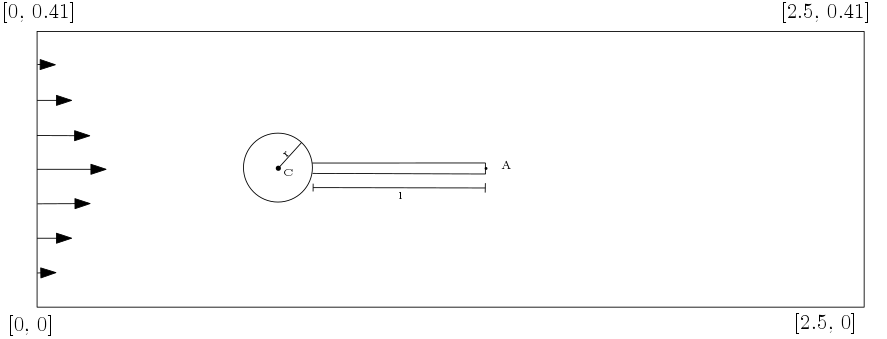
\includegraphics[scale=0.5]{./Fig/turekflag.png}
      \caption{Computational domain of the validation benchmark}
\end{figure}
\newpage


The benchmark is divided into three main test environments.
In the first environment the fluid solver is tested for a series of different flow profiles. The second environment regards the structure implementation, regarding bending of the elastic flag. And the final environment concerns validation the full fluid-structure interaction problem. The test environments are further divided into three different problems with increasing difficulty, posing different challenges to the implementation.

 Several quantites for comparion are presented in \cite{Hron2006} for validation purposes. 

\begin{itemize}
\item The position (x,y) of point A(t) as the elastic flag undergoes deformation.
\item Drag and lift forces exerted on of the whole interior geometry in contact with the fluid, consisting of the rigid circle and the elastic beam.
\begin{align*}
(F_D, F_L) = \int_{\Gamma} \mathbf{\sigma} \cdot \mathbf{n} dS
\end{align*}
\end{itemize}

The following environments and their sub-problems presents both steady state and periodic solutions. For the steady state solutions, the quantity of interest will be calculated for the last time step. For the periodic solutions, the amplitude and mean values for the time dependent quantity are calculated from the last period of oscillations.The mean value and amplitude is given by,
\begin{align*}
\text{mean} = \frac{1}{2} \text{max + min} \\
\text{amplitude} = \frac{1}{2} \text{max . min}
\end{align*}
from the maximum and minimum value of the quantity of interest from the last period.  

 In \cite{Hron2006}, all steady state solutions seems to be calulated by solving a steady state equation since time-step are only reported for the periodic solutions. In this thesis, all problems in \cite{Hron2006} are calculated by time integration. The main motivation is based upon that any given numerical errors regarding time integration will be intercepted at an earlier stage for a simpler problem. Therefore, the choice of time step  is chosen such that reasonable accuracy of the reference solution is attained.

 In the following section, an overview of each environment together with numerical results will be presented. A formal discussion of the results are given at the end of each simulation environment. For each table, the error of the finest spatial and temporal refinement compared to the reference solution is reported jn \cite{Hron2006} OTHER CITE.

 \newpage
\subsection{Validation of fluid solver}
The first test environment conserns the fluid dynamics part of the total FSI problem, to ensure the solver can handle flows in low Reynold-numbers regime. Two approaches for the validation are given in \cite{Hron2006}. The first approach considers setup as a fluid-structure interaction problem, by setting the elastic flag close to rigid  by manipulation of the structure parameters. In the second approach, the flag is set fully rigid and considered a purely flow problem.  Hence, the fluid variation formulation can be reduced to


Find $\bat{v}_f, \ha{p}_f $ such that
\begin{align*}
 \big( \pder{\bat{v}}{t}, \ \gat{\psi}^u \big)_{\hat{\Omega}_f} +
\femf{(\bat{v} \cdot \hat{\nabla}) \bat{v}}{\gat{\psi}^u}
- \femf{\hat{\sigma}}{\hat{\nabla}\gat{\psi}^u} -
\femf{\rho_f  \mathbf{f}_f}{{\gat{\psi}^u}} = 0 \\
\femf{\nabla \cdot \bat{v})}{\gat{\psi}^p} = 0 
\end{align*} 

The latter approach is chosen for this thesis, as only the variational formulation for the fluid is tested and removes any influence of the structure and mesh extrapolation discretization.  Since $\hat{\Omega}_f = {\Omega}_f(t) \hspace{2mm} t \in T$, the mesh velocity of the fluid $ \pder{\ha{T}_W}{t} = 0$  and no deformation of the fluid domain is present.

The validation of the fluid solver is divided into the three sub-cases; CFD1, CFD2, and CFD3. While  CFD1 and CFD2 yields steady state solutions, CFD3 is a periodic solution.

%\begin{figure}[h!]
  %\centering
    %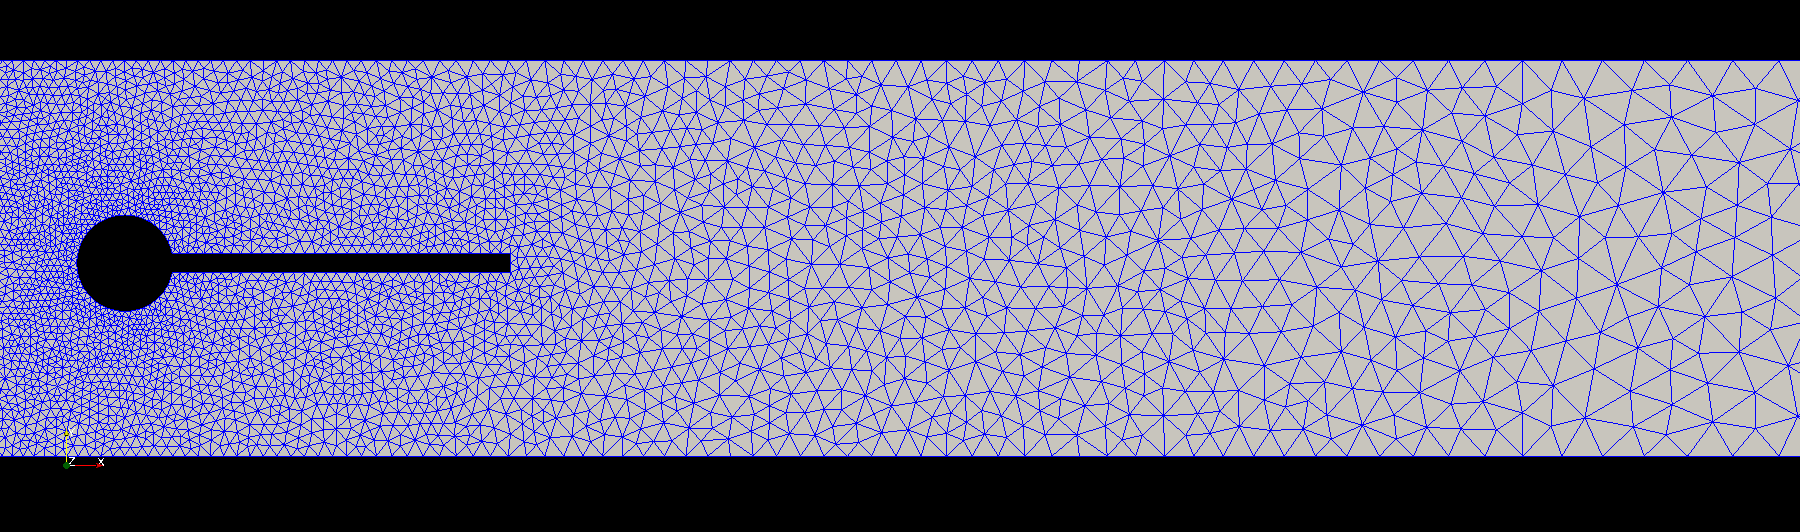
\includegraphics[scale=0.3]{./Fig/cfd1mesh.png}
      %\caption{Computational domain of channel flow with rigid inner geometry. }
%\end{figure}

\begin{table}[h!]
\centering
\caption{Benchmark environment}
\label{my-label}
\begin{tabular}{ |p{3cm}||p{2cm}|p{2cm}|p{2cm}|  }
 \hline
 \multicolumn{4}{|c|}{Fluid parameters} \\
 \hline
 parameter              & CFD 1 & CFD 2 & CFD 3 \\
 \hline
$\rho^f [10^{3}\frac{kg}{m^3}]$ & 1    & 1    & 1    \\
$\nu^f  [10^{-3}\frac{m^2}{s}]$  & 1    & 1    & 1    \\
U                      & 0.2  & 1    & 2    \\
Re                     & 20   & 100  & 200 \\
\hline
\end{tabular}
\end{table}

A parabolic velocity profile on the form,
\begin{align*}
v_f(0, y) = 1.5 U\frac{(H -y)y}{(\frac{H}{2})^2}
\end{align*}
is set on the left channel inflow. H is the height of the channel, while the parameter U is set differently to each problem to induce different inlet flow profiles. At the right channel outflow, the pressure is set to $p = 0$. No-slip boundary conditions for the fluid are enforced on the channel walls, and on the inner geometry consisting of the circle and the elastic flag. The validation is based on the evaluation of drag and lift forces on the inner geometry for each sub-case. Each sub-case will be conducted on four different mesh, with increasing refinement.  The following tables presents the numerical results for each sub-case.

\newpage

\begin{table}[h!]
\centering
\caption{CFD 1 Results}
\label{CFD 1 Results}
\begin{tabular}{ |p{1cm}||p{2.7cm}|p{3.3cm}|p{3.3cm}|}
\hline
  \multicolumn{4}{|c|}{$\Delta t = 0.1 \hspace{2mm} \theta = 1.0$} \\
\hline
nel & ndof & Drag  & Lift \\
\hline
 1438    & 6881   & 13.60 & 1.089  \\
 2899    & 13648  & 14.05 & 1.126 \\
 7501    & 34657  & 14.17   & 1.109 \\
 19365   & 88520  & 14.20 & 1.119 \\
  \hline
  \multicolumn{2}{|c|}{Reference}  & 14.29   & 1.119\\
   \hline
    \multicolumn{2}{|c|}{Error}  & 0.006 \%   & 0.00 \%\\
   \hline
\end{tabular}
\end{table}

\begin{table}[h!]
\centering
\caption{CFD-2}
\label{CFD-2 Results}
\begin{tabular}{ |p{1cm}||p{2.7cm}|p{3.3cm}|p{3.3cm}|}
 \hline
  \multicolumn{4}{|c|}{$\Delta t = 0.01 \hspace{2mm} \theta = 1.0$} \\
   \hline
nel & ndof & Drag  & Lift \\
\hline
 1438    & 6881 (P2-P1)  & 126.0 &  8.62 \\
 2899    & 13648  (P2-P1)& 131.8 & 10.89  \\
 7501    & 34657 (P2-P1) & 135.1 & 10.48  \\
 19365   & 88520(P2-P1)  & 135.7 & 10.55  \\
 \hline
  \multicolumn{2}{|c|}{Reference}  & 136.7   & 10.53\\
   \hline
    \multicolumn{2}{|c|}{Error}  & 0.007 \%   & 0.001 \%\\
   \hline
\end{tabular}
\end{table}

\begin{figure}[h!]
  \centering
    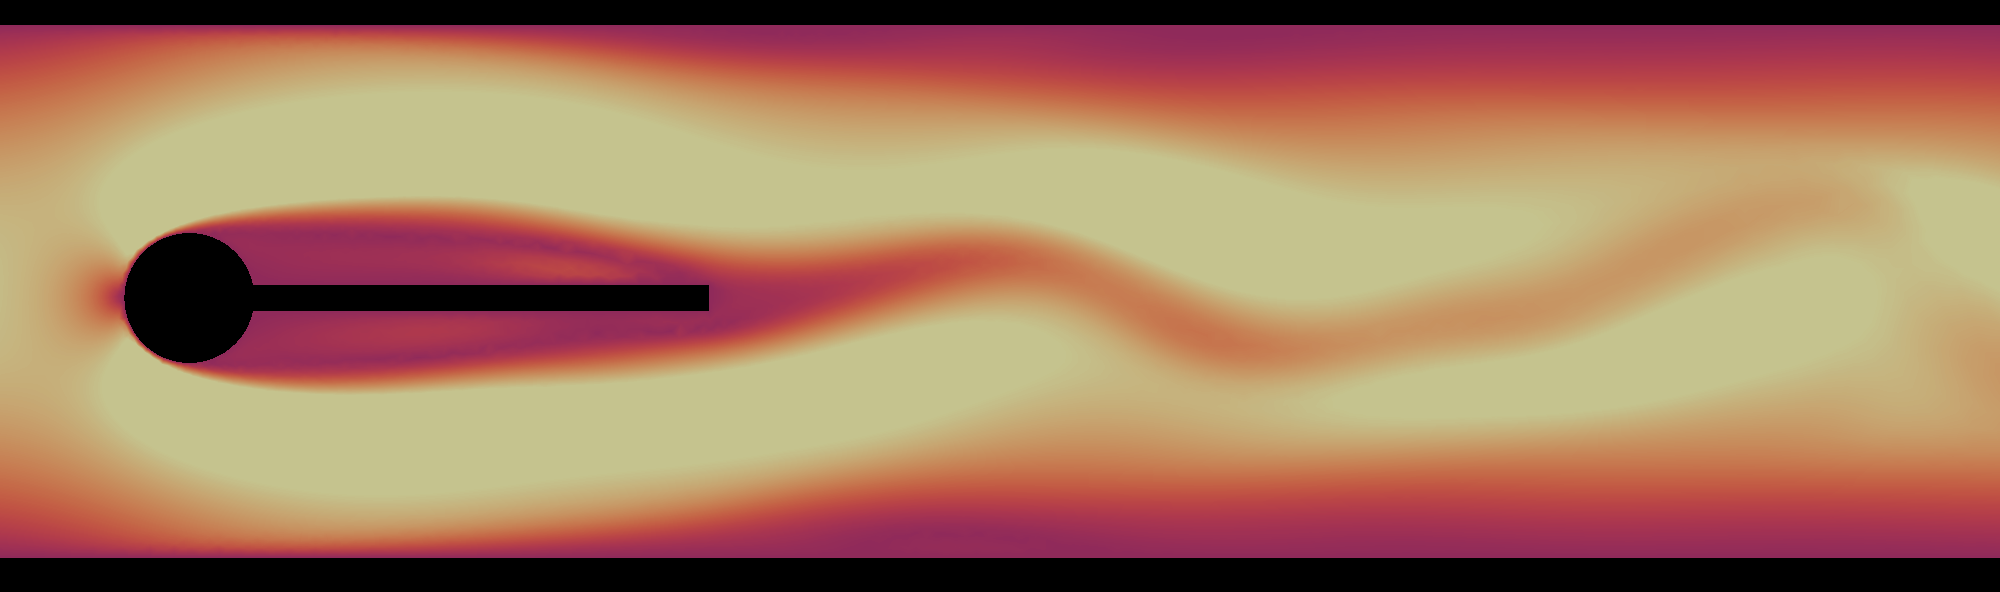
\includegraphics[scale=0.2]{./Fig/cfd3.png}
      \caption{CFD-3, flow visualization of velocity time t = 9s}
\end{figure}

\begin{figure}[h!]
  \centering
    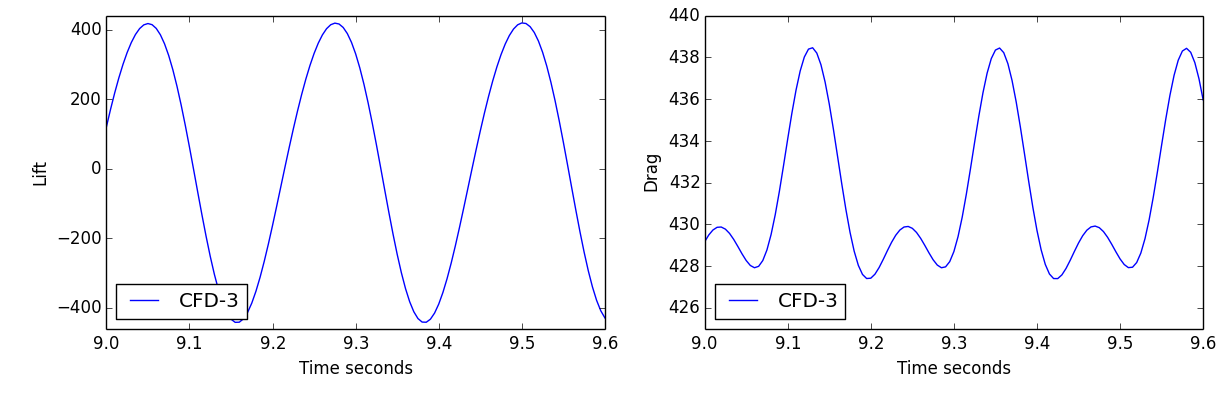
\includegraphics[scale=0.5]{./Fig/cfd3_liftdrag.png}
      \caption{CFD-3, lift and drag forces at time t = [9, 9.6]}
\end{figure}


\begin{table}[h!]
\centering
\caption{CFD-3}
\label{CFD-3 Results}
\begin{tabular}{ |p{1cm}||p{2.9cm}|p{3.3cm}|p{3.3cm}|}
 \hline
  \multicolumn{4}{|c|}{$\Delta t = 0.01 \hspace{2mm} \theta = 0.5$} \\
   \hline
nel & ndof & Drag  & Lift \\
\hline
 1438    & 6881  (P2-P1)   & 417.23       +/-  0.0217 & -249.21       +/-  0.32  \\
   & 16474 (P3-P2)   & 414.86      $\pm$  5.6282 & -7.458      $\pm$  444.07  \\
 \hline
 2899    & 13648  (P2-P1) & 408.50  $\pm$   4.3029 & -19.731  $\pm$   373.45 \\  
     &  32853 (P3-P2)  & 432.86      $\pm$  5.5025 & -9.686      $\pm$  431.28  \\
  \hline
  7501    & 34657 (P2-P1) & 431.57  $\pm$   5.2627 & -12.497  $\pm$   429.76 \\    
    &  83955 (P3-P2)  & 438.20      $\pm$  5.5994 & -11.595      $\pm$  438.00 \\
    \hline
    19365   & 88520 (P2-P1) & 435.43  $\pm$   5.4133 & -11.545  $\pm$   438.89 \\
   &   215219 (P3-P2) & 438.80      $\pm$  5.6290 & -11.158      $\pm$  439.23 \\
\hline
 \multicolumn{2}{|c|}{Reference}  & 439.95 $\pm$ 5.6183 & -11.893 $\pm$ 437.81\\
 \hline
  \multicolumn{2}{|c|}{Error}  & 0.002 \% $\pm$ 0.001 \% & 0.061 \% $\pm$ 0.003\% \\
  \hline
  \end{tabular}
  \vspace{2cm}
 \begin{tabular}{ |p{1cm}||p{2.9cm}|p{3.3cm}|p{3.3cm}|}
  \hline
  \multicolumn{4}{|c|}{$\Delta t = 0.005 \hspace{2mm} \theta = 0.5$} \\
   \hline
nel & ndof & Drag  & Lift \\
\hline
 1438    & 6881  (P2-P1)   &  417.24  $\pm$  0.0084 & -249.386   $\pm$ 0.1345  \\
 1438    & 16474 (P3-P2)   & 414.90     $\pm$  5.7319 & -8.467 $\pm$  443.45  \\
\hline
 1438    &13648  (P2-P1)   & 408.27   $\pm$ 4.0192 & -18.981   $\pm$ 363.84 \\
 2899    &  32853 (P3-P2)   & 432.90      $\pm$  5.5333 & -11.382      $\pm$  430.60 \\
 \hline
 1438    & 34657  (P2-P1)   & 431.59 $\pm$5.2979 & -13.644   $\pm$ 429.68 \\
 7501    & 83955 (P3-P2)  & 438.23      $\pm$  5.6393 & -12.917 $\pm$  437.78 \\
 \hline
 1438    & 88520  (P2-P1)   & 435.46  $\pm$ 5.4579 & -13.190   $\pm$ 438.05 \\
 19365   & 215219 (P3-P2)  & 438.84    $\pm$  5.6576 & -12.786      $\pm$  438.36 \\
\hline
 \multicolumn{2}{|c|}{Reference}  & 439.95 $\pm$ 5.6183 & -11.893 $\pm$ 437.81\\
 \hline
  \multicolumn{2}{|c|}{Error}  & 0.002 \% $\pm$ 0.006 \% & 0.075 \% $\pm$ 0.001\% \\
  \hline
\end{tabular}
\end{table}

\newpage \newpage \newpage \newpage \newpage
\subsection{Discussion of results}
The numerical results for CFD1, CFD2 and CFD3 are all within reasonable range of the reference solutions presented in \cite{Hron2006}. For CFD1 and CFD2, the choice of P2-P1 elements together with a fully implicit schene $\theta = 1$ gained sufficient accuracy in comparison with the reference solution. The second order cranc-nicholoson scheme  $\theta = 0.5$ was investigated for CFD1 and CFD2, however only improving the results of order $10^{-6}$ for both lift and drag. For the periodic problem CFD-3, the choice of  P2-P1 elements with a fully implicit time-stepping scheme proved unsufficient for capturing the expected periodic solution.  By cranc-nicolson time-stepping scheme $\theta = 0.5$, the periodic solution was attained. Since the choice of finite-elemt pair is not reported in the original work, both P3-P2 and P2-P1 element pairs for fluid and pressure respectively was compared in combination with spatial mesh refinement. From Table 1.4, the choice P3-P2 element pair is eminent to achieve reasonable results for the first and second mesh regardless of timestep.  However, the third and fourth mesh shows close resemblance with the reference solution. On this basis, the choice of P2-P1 element pair is sufficient for the evaluation of drag and lift on the inner geometry with increasing mesh resolution. 

\newpage
\subsection{Validation of solid solver}
\begin{table}[h!]
\centering
\caption{CSM validation environment}
\label{my-label}
\begin{tabular}{ |p{3cm}||p{2cm}|p{2cm}|p{2cm}|  }
 \hline
 \multicolumn{4}{|c|}{Fluid parameters} \\
 \hline
 parameter              & CSM 1 & CSM 2 & CSM 3 \\
 \hline
$\rho^s [10^{3}\frac{kg}{m^3}]$ & 1    & 1    & 1    \\
$\nu^s $  & 0.4    & 0.4    & 0.4    \\
$\mu^s  [10^{6}]$  & 0.5    & 2.0    & 0.5    \\
$g  \frac{m}{s^2}]$  & 2.0    & 2.0    & 2.0    \\
\hline
\end{tabular}
\end{table}

The validation of the solid solver is conducted on a rectangular domain, representing the elastic structure behind the circle in Figure ?.  The structure is submitted to a gravitational for $\mathbf{g} = (0, g)$, while beeing fixed to a fictional wall on the left side of the domain. The validation of the solid solver is based on comparison of the deflection of point $A(t) = [A_x(t), A_y(t)]$,  conducted on three refined mesh, where the number of finite elements are chosen in close resemblance with the original work in \cite{Hron2006}. A simple investigation of different finite-element pairs, suggest that P3-P3 elements where used for making the reference solution. In this study, lower order finite-element pair was included by the motivation of shorter simulation time while retaining solution accuracy. While computational time is not a major concern for the solid solver, the study is important for potentially reducing the computational time for the final validation environment.

\begin{table}[h!]
\centering
\caption{CSM 1 Results}
\label{CSM 1 Results}
\begin{tabular}{ |p{1cm}||p{2.7cm}|p{3.3cm}|p{3.3cm}|}
\hline
  \multicolumn{4}{|c|}{$\Delta t = 0.1 \hspace{2mm} \theta = 1.0$} \\
\hline
nel & ndof & ux of A [x $10^{3}$]  &uy of A [x $10^{3}$] \\
\hline
 319     & 832 P1-P1  & -5.278 &  -56.6 \\
     & 2936 P2-P2 & -7.056 &  -65.4 \\
      & 6316 P3-P3 &  -7.064 &   -65.5  \\
 \hline
  1365    & 3140 P1-P1  & -6.385 &  -62.2 \\
     & 11736 P2-P2 & -7.075 &  -65.5 \\
     & 25792 P3-P3 & -7.083 &  -65.5 \\
 \hline
  5143    & 11084 P1-P1 & -6.905 &  -64.7  \\
     & 42736 P2-P2 & -7.083 &  -65.4\\
     & 94960 P3-P3 & -7.085 &  -65.5  \\
  \hline
  \multicolumn{2}{|c|}{Reference}  &-7.187    & -66.1 \\
   \hline
    \multicolumn{2}{|c|}{Error}  & 1.41 \%   & 0.8 \%\\
   \hline
\end{tabular}
\end{table}

\begin{table}[h!]
\centering
\caption{CSM 2 Results}
\label{CSM 2 Results}
\begin{tabular}{ |p{1cm}||p{2.7cm}|p{3.3cm}|p{3.3cm}|}
\hline
  \multicolumn{4}{|c|}{$\Delta t = 0.05 \hspace{2mm} \theta = 1.0$} \\
\hline
nel & ndof & ux of A [x $10^{3}$]  &uy of A [x $10^{3}$] \\
\hline

 319     & 832 P1-P1  & -0.3401 &  -14.43  \\ 
     & 2936 P2-P2 &  -0.460  &  -16.78  \\ 
      & 6316 P3-P3 & -0.461 &  -16.79  \\
        \hline
  1365    & 3140 P1-P1  &  -0.414 &  -15.93\\
     & 11736 P2-P2 &  -0.461 &  -16.81 \\
     & 25792 P3-P3 & -0.461  &  -16.82 \\
        \hline
   5143    & 11084 P1-P1 & -0.449 &  -16.60  \\
     & 42736 P2-P2 &-0.461 &  -16.82 \\
     & 94960 P3-P3 & -0.462 &  -16.82 \\
  \hline
  \multicolumn{2}{|c|}{Reference}  & -0.469      & -16.97  \\
   \hline
    \multicolumn{2}{|c|}{Error}  & 1.49\%   & 0.88 \%\\
   \hline
\end{tabular}
\end{table}

\begin{table}[h!]
\centering
\caption{CSM 3 Results}
\label{CSM 3 Results}
\begin{tabular}{ |p{1cm}||p{2.7cm}|p{3.3cm}|p{3.3cm}|}
\hline
  \multicolumn{4}{|c|}{$\Delta t = 0.02 \hspace{2mm} \theta = 0.5$} \\
\hline
nel & ndof & ux of A [x $10^{3}$]  &uy of A [x $10^{3}$] \\
\hline
 319     & 832 P1-P1  & -10.790       +/-  10.797 & -55.184       +/-  56.682 \\
     & 2936 P2-P2 & -14.380       +/-  14.387 & -63.198       +/-  65.147 \\
      & 6316 P3-P3 & -14.409       +/-  14.417 & -63.288       +/-  65.225 \\
  \hline
   1365    & 3140 P1-P1 & -13.032       +/-  13.041 & -60.446       +/-  62.075 \\
     & 11736 P2-P2 & -14.407       +/-  14.416 & -63.283       +/-  65.220 \\
     & 25792 P3-P3 & -14.412       +/-  14.421 & -63.310       +/-  65.246 \\
   \hline
    5143    & 11084 P1-P1 & -14.059       +/-  14.071 & -62.591       +/-  64.473 \\
     & 42736 P2-P2  & -14.412       +/-  14.421 & -63.313       +/-  65.249 \\
     & 94960 P3-P3 & -14.416       +/-  14.425 & -63.328       +/-  65.263 \\
    \hline
  \multicolumn{2}{|c|}{Reference}  &-14.305 +- -14.305        & -63.607 +- 65.160    \\
   \hline
    \multicolumn{2}{|c|}{Error}  & \%   &  \%\\
   \hline
\end{tabular}
\end{table}

\begin{table}[h!]
\centering
%\caption{CSM 3 Results 2}
\label{CSM 3 Results 2}
\begin{tabular}{ |p{1cm}||p{2.7cm}|p{3.3cm}|p{3.3cm}|}
\hline
  \multicolumn{4}{|c|}{$\Delta t = 0.01 \hspace{2mm} \theta = 0.5$} \\
\hline
nel & ndof & ux of A [x $10^{3}$]  &uy of A [x $10^{3}$] \\
\hline
    319     & 832 P1-P1 & -10.835       +/-  10.836 & -55.197       +/-  56.845 \\
     & 2936 P2-P2 & -14.390       +/-  14.392 & -63.303       +/-  65.149 \\
      & 6316 P3-P3& -14.432       +/-  14.435 & -63.397       +/-  65.263 \\
    \hline
    1365    & 3140 P1-P1  & -13.053       +/-  13.054 & -60.367       +/-  62.241 \\
     & 11736 P2-P2  & -14.428       +/-  14.432 & -63.388       +/-  65.256 \\
     & 25792 P3-P3  & -14.444       +/-  14.446 & -63.432       +/-  65.287 \\
     \hline
     5143    & 11084 P1-P1 & -14.082       +/-  14.084 & -62.656       +/-  64.495 \\
     & 42736 P2-P2 & -14.444       +/-  14.447 & -63.435       +/-  65.288 \\
     & 94960 P3-P3& -14.449       +/-  14.452 & -63.449       +/-  65.296 \\
 \hline
  \multicolumn{2}{|c|}{Reference}  &-14.305 +- -14.305        & -63.607 +- 65.160    \\
   \hline
    \multicolumn{2}{|c|}{Error}  & \%   &  \%\\
   \hline
\end{tabular}
\end{table}


\begin{table}[h!]
\centering
%\caption{CSM 3 Results 3}
\label{CSM 3 Results 3}
\begin{tabular}{ |p{1cm}||p{2.7cm}|p{3.3cm}|p{3.3cm}|}
\hline
  \multicolumn{4}{|c|}{$\Delta t = 0.005 \hspace{2mm} \theta = 0.5$} \\
\hline
nel & ndof & ux of A [x $10^{3}$]  &uy of A [x $10^{3}$] \\
\hline
    319     & 832 P1-P1 & -10.846       +/-  10.848 & -56.049       +/-  56.053 \\
     & 2936 P2-P2  & -14.390       +/-  14.391 & -63.738       +/-  64.703 \\
      & 6316 P3-P3 & -14.429       +/-  14.430 & -63.833       +/-  64.810 \\
 \hline 
    1365    & 3140 P1-P1 & -13.057       +/-  13.057 & -60.813       +/-  61.826 \\
     & 11736 P2-P2& -14.426       +/-  14.427 & -63.827       +/-  64.801 \\
     & 25792 P3-P3 & -14.440       +/-  14.441 & -63.854       +/-  64.845 \\
 \hline
      5143    & 11084 P1-P1 & -14.091       +/-  14.091 & -63.195       +/-  63.981 \\
     & 42736 P2-P2 & -14.441       +/-  14.441 & -63.856       +/-  64.847 \\
     & 94960 P3-P3 & -14.446       +/-  14.446 & -63.865       +/-  64.860 \\
 \hline
  \multicolumn{2}{|c|}{Reference}  &-14.305 +- -14.305        & -63.607 +- 65.160    \\
   \hline
    \multicolumn{2}{|c|}{Error}  & \%   &  \%\\
   \hline
\end{tabular}
\end{table}

\begin{figure}[h!]
  \centering
    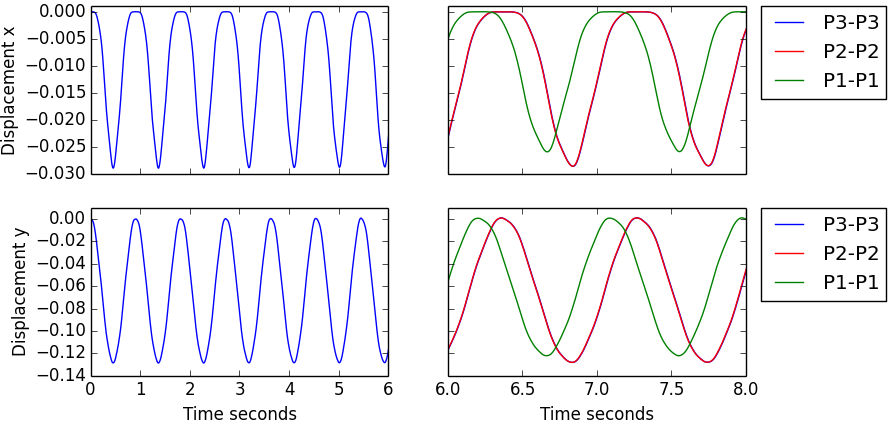
\includegraphics[scale=0.6]{./Fig/csm3compare.png}
      \caption{CSM-3, deformation components of A(t) for two different time intervals. Time interval $t \in [0, 6]$ shows the P3-P3 element pair, while$t \in [6, 8]$ compares all finite elemet pair chosen for the experiment}
\end{figure}

\subsection{Discussion of results}
The results for sub-problems CSM-1 and CSM-2 each coincide with the reference solution. The study of lower-grade elements proved successful for both problems, justifying accurate results can be achieved for polynomials grade 1 and 2 for all mesh refinements. This observation is further justified in the CSM-3 results. In table 1.4, the  displacement components of P3-P3 and P2-P2 elements can hardly be distinguished.


\newpage
\subsection{Validation of fluid structure interaction solver}
The validation of the FSI solver constist of three sub-cases which will be referred to FSI-1, FSI-2 and FSI-3. The FSI-1 environment yields a steady state solution for the system, inducing small deformations to the elastic flag. This environment is excellent to ensure the overall coupling of the FSI-problem is executed properly. The FSI-2 and FSI-3 environment results in a periodic solution, where the elastic flag oscilates behind the sylinder.


 For all sub-cases
a parabolic velocity profile on the form,
\begin{align*}
v_f(0, y) = 1.5 U\frac{(H -y)y}{(\frac{H}{2})^2}
\end{align*}
is set on the left channel inflow. H is the height of the channel, while the parameter U is set differently to each problem to induce different flow profiles. \
At the right channel outflow, the pressure is set to $p = 0$. \
No-slip boundary conditions for the fluid are enforced on the channel walls, and on the circle of the inner geometry.
The structure deformation and velocity is set to zero on the left side of the flag, where the flag is ancored to the circle. On the fluid-structure interface $\Gamma$, we enfore the kinematic and dynamic boundary condition
\begin{align}
\mathbf{v}_f = \mathbf{v}_s \\
\mathbf{\sigma}_f \cdot \mathbf{n} = \mathbf{\sigma}_s \cdot \mathbf{n}
\end{align}
From chapter ?,  (1.1) is enforced strongly due to the continious velocity field, while (1.2) is enforced weakly by omtitting form the weak formulation by.



Apart from the accuracy of the reported values, the main purpose of the validation of the fluid solver is twofold. Firstly, it is of great importance to ensure that the overall coupling of the fluid-structure interaction problem are executed correctly. Second, a good choice of mesh extrapolation model is essential to ensure that mesh entanglement is not present. Based on the experience with the previous sub-problems, the finite element group of P2-P2-P1 is chosen for deformation, velocity and pressure  . 


\begin{table}[h!]
\centering
\caption{Benchmark environment}
\label{my-label}
\begin{tabular}{ |p{3cm}||p{2cm}|p{2cm}|p{2cm}|  }
 \hline
 \multicolumn{4}{|c|}{Solid parameters} \\
 \hline
 parameter              & FSI1 & FSI2 & FSI3 \\
 \hline
 $\rho^s [10^{3} \frac{kg}{m^3}]$ & 1    & 10   & 1    \\
$\nu^s$ & 0.4  & 0.4  & 0.4  \\
$\mu^s  [10^{6}\frac{kg}{ms^2}]$  & 0.5  & 0.5  & 2.0  \\
 \hline
 \multicolumn{4}{|c|}{Fluid parameters} \\
 \hline
$\rho^f [10^{3}\frac{kg}{m^3}]$ & 1    & 1    & 1    \\
$\nu^f  [10^{-3}\frac{m^2}{s}]$  & 1    & 1    & 1    \\
U                      & 0.2  & 1    & 2    \\
parameter              & FSI1 & FSI2 & FSI3 \\
Re                     & 20   & 100  & 200 \\
\hline
\end{tabular}
\end{table}

\newpage
\subsubsection{FSI1}


\begin{table}[h!]
\centering
\caption{FSI 1 Results}
\label{FSI1 Results}
\begin{tabular}{ |p{1cm}||p{1cm}|p{2.5cm}|p{2.5cm}|p{2.7cm}|p{2.7cm}|p{1.2cm}|}
 \hline
  \multicolumn{6}{|c|}{Laplace} \\
   \hline
nel & ndof & ux of A [x $10^{3}$]  &uy of A [x $10^{3}$]& Drag  & Lift \\
 \hline
 2474    & 21249  &       0.0226 &       0.8200 & 14.061 & 0.7542 \\
 7307    & 63365  &       0.0227 &       0.7760 & 14.111 & 0.7517 \\
 11556   & 99810  &       0.0226 &      0.8220 & 14.201 & 0.7609 \\
  \hline
 \multicolumn{2}{|c|}{Reference} &  0.0227      &       0.8209      & 14.295  & 0.7638   \\
 \hline
\end{tabular}
\begin{tabular}{ |p{1cm}||p{1cm}|p{2.5cm}|p{2.5cm}|p{2.7cm}|p{2.7cm}|p{1.2cm}|}
 \hline
  \multicolumn{6}{|c|}{Linear Elastic} \\
   \hline
nel & ndof & ux of A [x $10^{3}$]  &uy of A [x $10^{3}$]& Drag  & Lift \\
 \hline
 2474    & 21249  &       0.0226 &       0.8198 & 14.061 & 0.7541 \\
 7307    & 63365  &       0.0227 &       0.7762 & 14.111 & 0.751  \\
 11556   & 99810  &       0.0226  &       0.8222 & 14.201 & 0.7609 \\
  \hline
 \multicolumn{2}{|c|}{Reference} &  0.0227      &       0.8209      & 14.295  & 0.7638   \\
 \hline
\end{tabular}
\begin{tabular}{ |p{1cm}||p{1cm}|p{2.5cm}|p{2.5cm}|p{2.7cm}|p{2.7cm}|p{1.2cm}|}
 \hline
  \multicolumn{6}{|c|}{Biharmonic bc1} \\
   \hline
nel & ndof & ux of A [x $10^{3}$]  &uy of A [x $10^{3}$]& Drag  & Lift \\
 \hline
 2474    & 21249  &       0.0226 &       0.8200 & 14.061 & 0.7541 \\
 7307    & 63365  &       0.0227  &       0.7761 & 14.111 & 0.7517 \\
 11556   & 99810  &       0.0227  &       0.8017 & 14.205 & 0.9248 \\
  \hline
 \multicolumn{2}{|c|}{Reference} &  0.0227      &       0.8209      & 14.295  & 0.7638   \\
 \hline
\end{tabular}
\begin{tabular}{ |p{1cm}||p{1cm}|p{2.5cm}|p{2.5cm}|p{2.7cm}|p{2.7cm}|p{1.2cm}|}
 \hline
  \multicolumn{6}{|c|}{Biharmonic bc2} \\
   \hline
nel & ndof & ux of A [x $10^{3}$]  &uy of A [x $10^{3}$]& Drag  & Lift \\
 \hline
 2474    & 21249  &       0.0226 &       0.8200 & 14.061 & 0.7543 \\
 7307    & 63365  &       0.0227 &       0.7761 & 14.111 & 0.7518 \\
 11556   & 99810  &       0.0227 &       0.8020 & 14.205 & 0.9249  \\
  \hline
 \multicolumn{2}{|c|}{Reference} &  0.0227      &       0.8209      & 14.295  & 0.7638   \\
 \hline
\end{tabular}
\end{table}


\begin{table}[h!]
\centering
\caption{FSI 1 - No extrapolation}
\label{FSI1- No extrapolation}
\begin{tabular}{ |p{1cm}||p{1cm}|p{2.5cm}|p{2.5cm}|p{2.7cm}|p{2.7cm}|p{1.2cm}|}
 \hline
  \multicolumn{6}{|c|}{No extrapolation} \\
   \hline
nel & ndof & ux of A [x $10^{3}$]  &uy of A [x $10^{3}$]& Drag  & Lift \\
 \hline
 2474    & 21249  &       0.0224 &       0.9008 & 14.064 & 0.7713 \\
 7307    & 63365  &       0.0226  &       0.8221 & 14.117 & 0.7660 \\
 11556   & 99810  &       0.0225 &       0.8787 & 14.212 & 0.7837 \\
  \hline
 REF     & REF    &       0.0227      &       0.8209      & 14.295  & 0.7638   \\
 \hline
\end{tabular}

\end{table}




\newpage \newpage
\subsubsection{FSI2}
FSI2
\begin{figure}[h!]
  \centering
    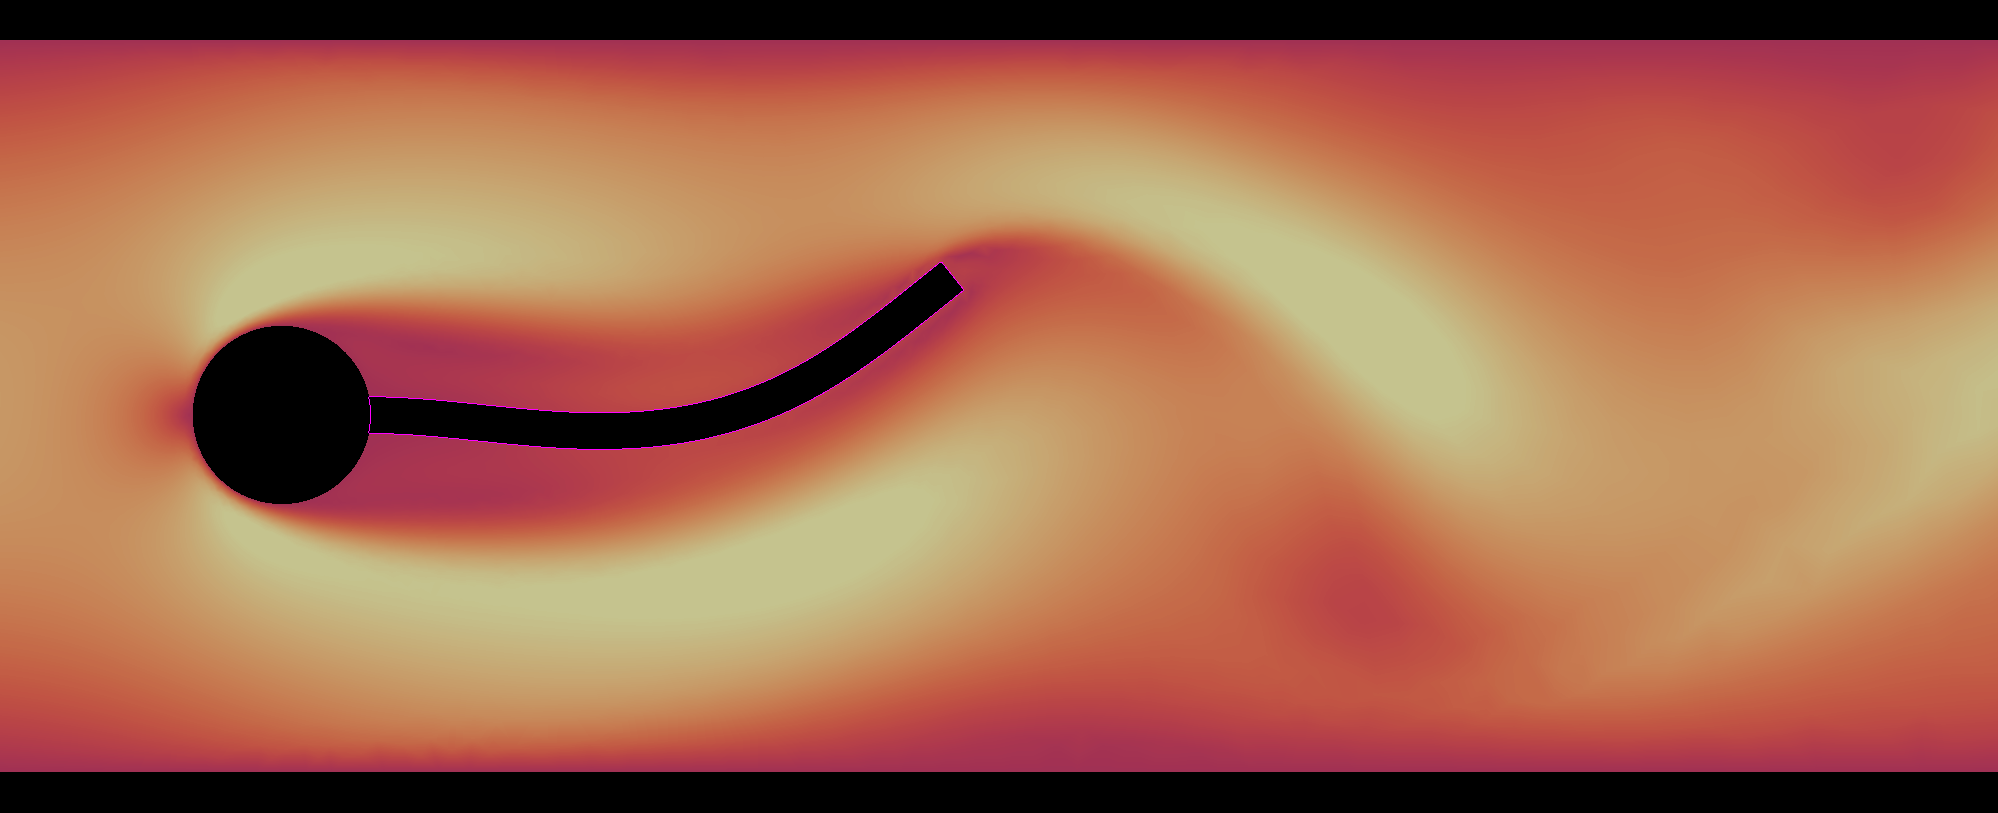
\includegraphics[scale=0.2]{./Fig/fsi2flow.png}
      \caption{FSI-2, visualization of fully developted flow with structure deformation at time t = 9s}
\end{figure}

\newpage
\subsubsection{FSI3}

\begin{table}[h!]
\centering
\caption{FSI 3 - Comparison of mesh extrapolation models}
\label{my-label}
\begin{tabular}{ |p{1cm}||p{1cm}|p{2.5cm}|p{2.5cm}|p{2.7cm}|p{2.7cm}|p{1.2cm}|}
 \hline
  \multicolumn{6}{|c|}{Laplace \hspace{2mm} $\Delta t = 0.01 \theta = 0.51$} \\
   \hline
nel & ndof & ux of A [x $10^{3}$]  &uy of A [x $10^{3}$]& Drag  & Lift \\
 \hline
 2474    & 21249  & -2.41      $\pm$ 2.41 & 1.49       $\pm$ 3.22 & 449.40       $\pm$ 14.70 & 0.55       $\pm$ 155.80  \\
 7307    & 63365  & -2.32       $\pm$ 2.30 & 1.34       $\pm$ 3.17 & 451.78       $\pm$ 16.08 & 1.13       $\pm$ 151.22  \\
 11556   & 99810  & -2.34       $\pm$ 2.34 & 1.57       $\pm$ 3.19 & 455.92       $\pm$ 17.32 & -0.10       $\pm$ 151.03 \\
 \hline
  \multicolumn{6}{|c|}{$\Delta t = 0.001 \theta = 0.501$} \\
   \hline
 nel & ndof & ux of A [x $10^{3}$]  &uy of A [x $10^{3}$]& Drag  & Lift \\
    \hline
1216 &5797& --2.17$\pm$  2.08 &     3.32     $\pm$  29.07 &439.98 $\pm$  14.08  &  1.91 $\pm$  151.71\\
2295 &10730& -3.04 $\pm$  2.88 &  1.51  $\pm$  35.88 & 452.04  $\pm$  22.41 &  3.30      $\pm$  160.11 \\
5963 &27486 & -3.03$\pm$  2.85 &  1.23 $\pm$  35.97  & 459.45  $\pm$  23.80 &  1.53  $\pm$  160.14 \\
 \hline
  \multicolumn{2}{|c|}{Reference}  & 136.7   & 10.53 & &\\
   \hline
    \multicolumn{2}{|c|}{Error}  & 0.007 \%   & 0.001 \% & &\\
   \hline
\end{tabular}
\end{table}

\begin{table}[h!]
\centering
%\caption{FSI 3 - Biharmonic BC1}
\label{my-label}
\begin{tabular}{ |p{0.9cm}||p{0.9cm}|p{2.49cm}|p{2.49cm}|p{2.6cm}|p{2.8cm}|}
 \hline
  \multicolumn{6}{|c|}{Biharmonic 1 \hspace{2mm}  $\Delta t = 0.01 \theta = 0.51$} \\
   \hline
nel & ndof & ux of A [x $10^{3}$]  &uy of A [x $10^{3}$]& Drag  & Lift \\
 \hline
 %2474    & 21249 & 7.96  $\pm$ 8.10  & -3.84   $\pm$ 1.02 & 450.16  $\pm$ 15.11 & $-20.09 \pm 148.17 $\\
 2474     &21249  &7.96  $\pm$ 8.10  &  -3.84   $\pm$ 1.02 & 450.16  $\pm$ 15.11  & -20.09 $\pm$ 148.17 \\
 7307    & 63365  & 3.10  $\pm$ 3.06  & -1.90   $\pm$ 4.21 & 457.37  $\pm$ 15.24 & -51.77 $\pm$ 127.28 \\
 11556   & 99810  & -2.18  $\pm$ 9.65 & 1.31    $\pm$ 4.93  & 456.40 $\pm$ 17.45 &  0.45 $\pm$ 149.68  \\
 \hline
  \multicolumn{6}{|c|}{$\Delta t = 0.001 \theta = 0.5$} \\
   \hline
 nel & ndof & ux of A [x $10^{3}$]  &uy of A [x $10^{3}$]& Drag  & Lift \\
1216 &5797  & -2.18       $\pm$ 2.10 & 3.56   $\pm$ 2.90 & 435.19       $\pm$ 9.77  & -1.57       $\pm$ 151.43 \\
7307    & 63365  & -1.42  $\pm$ 4.70 & 7.77   $\pm$ 2.85 & 454.38       $\pm$ 19.75 & 17.97       $\pm$ 155.08 \\
11556   & 99810  & -2.23  $\pm$ 6.16 & 1.72   $\pm$ 4.48 & 459.12       $\pm$ 22.97 & -3.12       $\pm$ 171.22 \\
 \hline
 \multicolumn{2}{|c|}{Reference} & -2.69 $\pm$  2.56                    & 1.48  $\pm$  34.38                   & 457.3  $\pm$  22.66        & 2.22  $\pm$- 149.78           \\
 \hline
 \multicolumn{2}{|c|}{Error}  & 0.007 \%   & 0.001 \% & &\\
 \hline
\end{tabular}
\end{table}

\begin{table}[h!]
\centering
%\caption{FSI 3 - Biharmonic BC2}
\label{my-label}
\begin{tabular}{ |p{1cm}||p{1cm}|p{2.5cm}|p{2.5cm}|p{2.7cm}|p{2.7cm}|p{1.2cm}|}
 \hline
  \multicolumn{6}{|c|}{Biharmonic 2 \hspace{2mm}  $\Delta t = 0.01 \theta = 0.51$} \\
   \hline
nel & ndof & ux of A [x $10^{3}$]  &uy of A [x $10^{3}$]& Drag  & Lift \\
 \hline
1216 &5797& -1.74  $\pm$  1.76 & 3.56 $\pm$  26.01 & 439.41$\pm$ 12.21  & -1.35    $\pm$  138.74\\
2295 &10730 & -2.39   $\pm$  2.40 &  1.76  $\pm$  32.27 & 449.71$\pm$ 18.16 &  3.71   $\pm$  149.97\\
 \hline
  \multicolumn{6}{|c|}{$\Delta t = 0.001 \theta = 0.501$} \\
   \hline
 nel & ndof & ux of A [x $10^{3}$]  &uy of A [x $10^{3}$]& Drag  & Lift \\
 1216 &5797& -3.39   $\pm$  3.38 &   1.23   $\pm$  36.61 &   413.26 $\pm$  51.82  &   57.19  $\pm$  222.65\\
 2295 &10730& -4.70  $\pm$  4.71& 1.49       $\pm$  44.62& 427.91$\pm$  93.17 &  44.38  $\pm$  268.05 \\
 \hline
 \multicolumn{2}{|c|}{Reference} & -2.69 $\pm$  2.56                    & 1.48  $\pm$  34.38                   & 457.3  $\pm$  22.66        & 2.22  $\pm$- 149.78           \\
 \hline
 \multicolumn{2}{|c|}{Error}  & 0.007 \%   & 0.001 \% & &\\
 \hline
\end{tabular}
\end{table}


\begin{figure}[h!]
    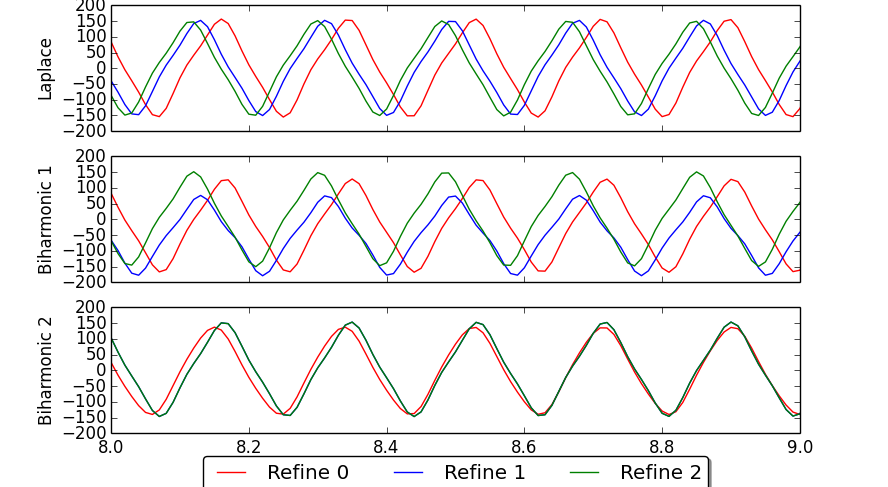
\includegraphics[scale=0.75]{./Fig/fsi3liftcompare.png}
      \caption{Comparing mesh extrapolation models}
\end{figure}

\begin{figure}[h!]
  \centering
    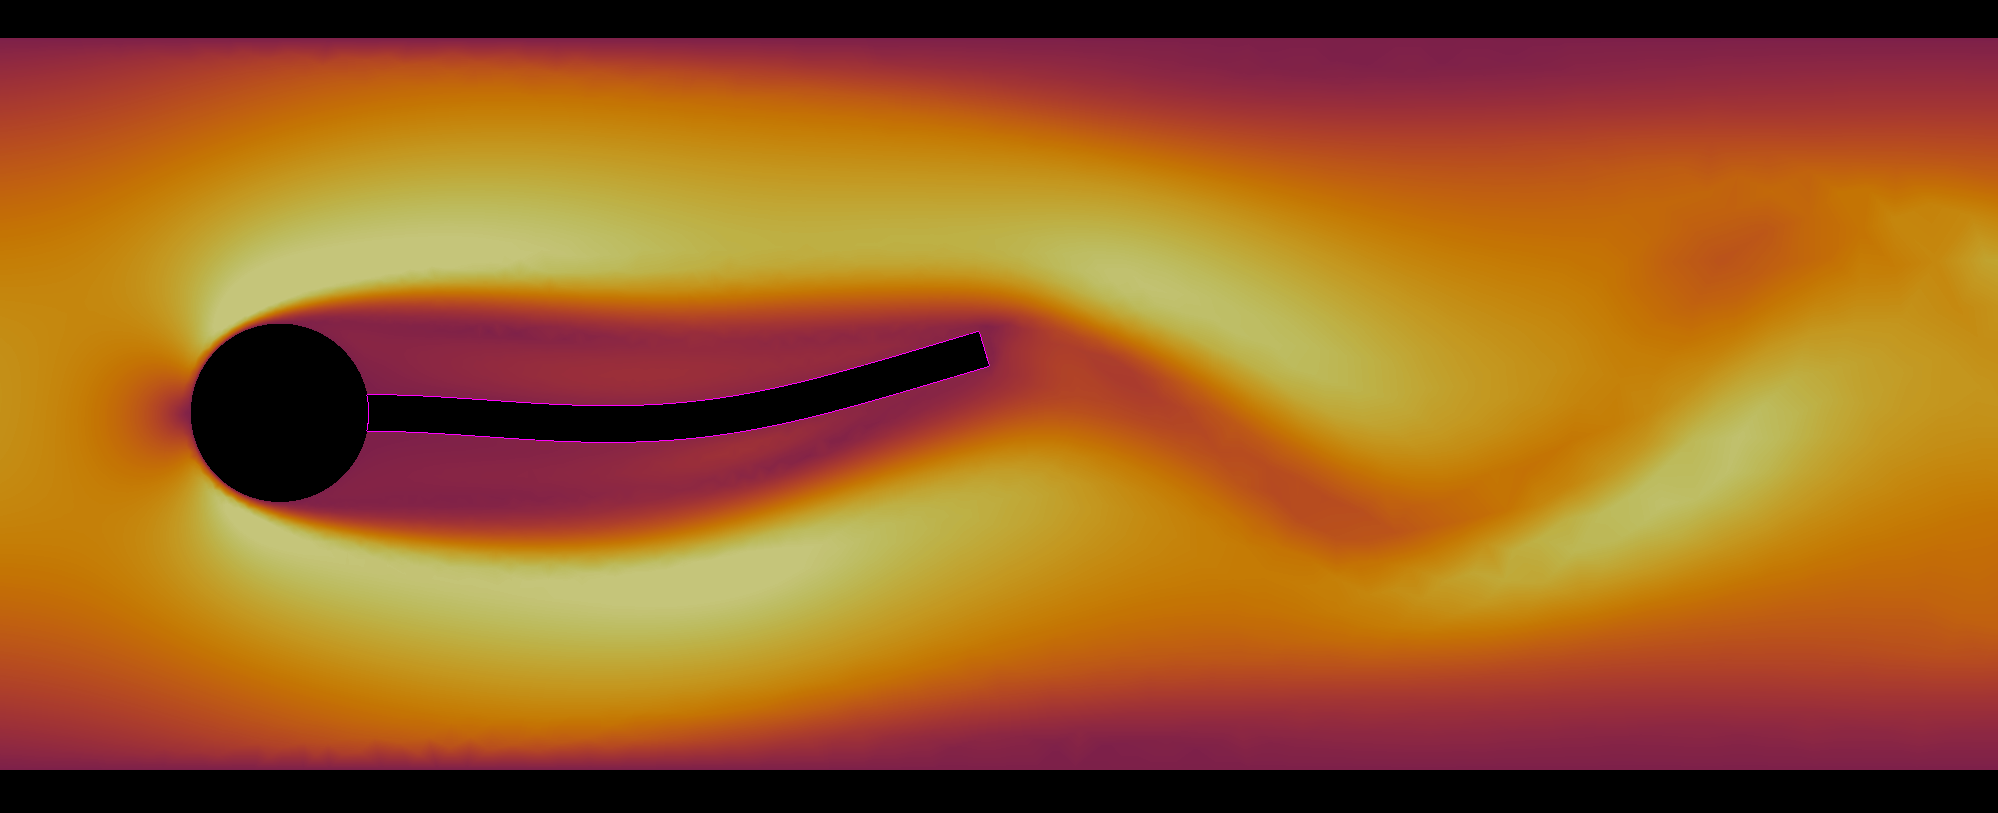
\includegraphics[scale=0.2]{./Fig/fsi3flow.png}
      \caption{FSI-3, visualization of fully developted flow with structure deformation at time t = 5.1s}
\end{figure}

\newpage
\subsection{Discussion of results}
Considering FSI1, all mesh extraplation models are of high accuracy compared to the reference solution.  However, due to the small deformations of order $10^{-6}$, FSI1 doesn't provide a rigorous test of the chosen mesh extrapolation model. By omitting mesh extrapolation from the variatonal formulation,  reasonable results are still obtained. This proves that the FSI-1 validation case can be misguiding, in terms of validating the chosen mesh extrapolation model. 

The FSI2 case proved to be one of the most demanding tests, due to the large deformation of the elastic flag. leading to the risk of entangled mesh cells. Therefore a high quality extrapolation of the solid deformation into the fluid is needed. All mesh extrapolation models proved to

The FSI3 environment does not induce deformation to the extent of the FSI2. However a critical phase in the transition to the periodic solution was discovered, where the pressure oscillation induces a large deformation to the system.










 


%\chapter{Implementation of Fluid Structure Interaction}

For the general monolithic FSI problem, several complexities arise considering discretization. Yet divided, both the fluid and structure problem themselves impose rather difficult problems. These in combination with the coupling of the two sub-problems and their interaction to one another, makes even the most simplest implementation surprisingly difficult.  \\
Both problem 4.1, 4.2 introduces several non-linear contributions to the governing equations. Firstly the more familiar terms from the convection term of the fluid equation, and the stress tensor of the structure model. Second, the ALE method introduces an additional domain-velocity term to the advection in the fluid problem,  were spatial differential operators and time derivatives depending on other variables of interest. 
Nevn papers hvor investigations of term has been made.

\begin{prob}
\textit{ALE term}\begin{align*}
\ha{J} (\hat{F}_W^{-1}(\bat{v} - \pder{\ha{T}_W}{t}) \cdot \hat{\nabla}) \bat{v}
\end{align*}
\text{for the first type of boundary conditions introduced. } 
\end{prob}
The stability of the time-stepping have proven to be affected by the ALE advection term, which is difficult to control CITE(formaggia). This chapter will focus on the mentioned introduced problems by the monolithic ALE method. A brief description will be given for the most central components and technologies used for this thesis.   

\section{FEniCS}
The main component of this thesis is the FEniCS project, an open-source finite element environment for solving partial differential equations (https://fenicsproject.org/). Using a combination of high-level Python and C++ interfaces, mathematical models can be implemented compactly and efficiently. FEniCS consists of several sub-modules and we will give a brief overview of the most central components used during implementation and computation.

\subsection{DOLFIN}
DOLFIN is the computational C++ backend of the FEniCS project, and the main user interface. It unifies several FEniCs components for implementing of computational mesh, function spaces, functions and finite element assembly. 

\begin{itemize} 
\item UFL (The Unified Form Language)  is a domain specific language, used for the discretization of mathematical abstractions of partial differential equations on a finite element form. Its implementation on top of Python, makes it excellent to define problems close to their mathematical notation without the use of more complex features. One uses the term \textit{form} to define any representation of some mathematical problem defined by UFL.   

\item FFC (The form compiler) compiles the finite elements variation forms given by UFL, generating low-level efficient C++ code 

\item FIAT the finite element backend, covering a wide range of finite element basis functions used in the discretization of of the  the finite-element forms. It covers a wide range of finite element basis functions for lines, triangles and tetrahedras.

\end{itemize}  


DOLFIN also incorporate the necessary interfaces to external linear algebra solvers and data structures. Within FEniCS terminology these are called linear algebra backends. PETSc is the default setting in FEniCS, a powerful linear algebra library
with a wide range of parallel linear and nonlinear solvers and efficient as matrix and vector operations for applications written in C, C++, Fortran and Python.
\newpage

\section{Implementation}
As implementation of mathematics differ from the choices of programming languages and external libraries, a deep dive within the implementation in FEniCS will not be covered in this thesis. Only variational forms and solvers will be presented as to give the reader a general overview of the key concept and the interpretation of mathematics. Basic knowledge of coding is assumed of the reader. 

\subsection{Variational Form}
Implementation of the code-blocks of the fluid variational form given in Chapter 3, and Newton solver will be presented. It is not the intention to give the reader a deep review of the total implementation, but rather briefly point out key ideas intended for efficient speedup of the calculation. These ideas have proven essential as for the reduction of computation time of the complex problem.

\begin{python}[caption=thetaCN.py]
def F_(U):
	return Identity(len(U)) + grad(U)

def J_(U):
	return det(F_(U))

def sigma_f_u(u,d,mu_f):
    return  mu_f*(grad(u)*inv(F_(d)) + inv(F_(d)).T*grad(u).T)

def sigma_f_p(p, u):
    return -p*Identity(len(u))

def A_E(J, v, d, rho_f, mu_f, psi, dx_f):
    return rho_f*inner(J*grad(v)*inv(F_(d))*v, psi)*dx_f \
        + inner(J*sigma_f_u(v, d, mu_f)*inv(F_(d)).T, grad(psi))*dx_f


def fluid_setup(v_, p_, d_, n, psi, gamma, dx_f, ds, mu_f, rho_f, k, dt, v_deg, theta, **semimp_namespace):

	J_theta = theta*J_(d_["n"]) + (1 - theta)*J_(d_["n-1"])
	F_fluid_linear = rho_f/k*inner(J_theta*(v_["n"] - v_["n-1"]), psi)*dx_f

	F_fluid_nonlinear =  Constant(theta)*rho_f*inner(J_(d_["n"])*grad(v_["n"])*inv(F_(d_["n"]))*v_["n"], psi)*dx_f
	F_fluid_nonlinear += inner(J_(d_["n"])*sigma_f_p(p_["n"], d_["n"])*inv(F_(d_["n"])).T, grad(psi))*dx_f
	F_fluid_nonlinear += Constant(theta)*inner(J_(d_["n"])*sigma_f_u(v_["n"], d_["n"], mu_f)*inv(F_(d_["n"])).T, grad(psi))*dx_f
	F_fluid_nonlinear += Constant(1 - theta)*inner(J_(d_["n-1"])*sigma_f_u(v_["n-1"], d_["n-1"], mu_f)*inv(F_(d_["n-1"])).T, grad(psi))*dx_f
	F_fluid_nonlinear +=inner(div(J_(d_["n"])*inv(F_(d_["n"]))*v_["n"]), gamma)*dx_f
	F_fluid_nonlinear += Constant(1 - theta)*rho_f*inner(J_(d_["n-1"])*grad(v_["n-1"])*inv(F_(d_["n-1"]))*v_["n-1"], psi)*dx_f
	F_fluid_nonlinear -= rho_f*inner(J_(d_["n"])*grad(v_["n"])*inv(F_(d_["n"]))*((d_["n"]-d_["n-1"])/k), psi)*dx_f

	return dict(F_fluid_linear = F_fluid_linear, F_fluid_nonlinear = F_fluid_nonlinear)
\end{python}

Alorithm 1.1 presents the implementation of the fluid residue, used in the Newton iterations. Apart from the rather lengthy form of the fluid residual, the strength of Unified Form Language preserving the abstract formulation of the problem is clear. The overall representation of the problem is by now just a form, its a representation and does not yet define vectors or matrices.

\begin{python}[caption=newtonsolver.py]
def newtonsolver(F, J_nonlinear, A_pre, A, b, bcs, \
              dvp_, up_sol, dvp_res, rtol, atol, max_it, T, t, **monolithic):
    Iter      = 0
    residual   = 1
    rel_res    = residual
    lmbda = 1

    while rel_res > rtol and residual > atol and Iter < max_it:
        if Iter % 4  == 0:
            A = assemble(J_nonlinear, tensor=A, form_compiler_parameters = {"quadrature_degree": 4}) 
            A.axpy(1.0, A_pre, True)
            A.ident_zeros()

        b = assemble(-F, tensor=b)

        [bc.apply(A, b, dvp_["n"].vector()) for bc in bcs]
        up_sol.solve(A, dvp_res.vector(), b)
        dvp_["n"].vector().axpy(lmbda, dvp_res.vector())
        [bc.apply(dvp_["n"].vector()) for bc in bcs]
        rel_res = norm(dvp_res, 'l2')
        residual = b.norm('l2')
        if isnan(rel_res) or isnan(residual):
            print "type rel_res: ",type(rel_res)
            t = T*T

\end{python}
\section{Optimization of Newtonsolver}
As for any program, the procedure of optimization involves finding the bottleneck of the implementation. Within computational science, this involves finding the area of code which is the primary consumer of computer resources. \\
As for many other applications, within computational science one can often assume the consummation of resources follows the \textit{The Pareto principle}. Meaning that for different types of events, roughly 80\% of the effects come from 20\% of the causes. An analogy to computational sciences it that 80\% of the computational demanding operations comes from 20\% of the code. In our case, the bottleneck is the newtonsolver. The two main reasons for this is 

\begin{itemize}
\item \textbf{Jacobian assembly} \\
The construction of the Jacobian matrix for the total residue of the system, is the most time demanding operations within the whole computation. 
\item \textbf{Solver}. \\ 
As iterative solvers are limited for the solving of fluid-structure interaction problems, direct solvers was implemented for this thesis. As such, the operation of solving a linear problem at each iteration is computational demanding, leading to  less computational efficient operations. Mention order of iterations?
\end{itemize}

Facing these problems, several attempts was made to speed-up the implementation. The FEniCS project consist of several nonlinear solver backends, were fully user-customization option are available. However one main problem which we met was the fact that FEniCS assembles the matrix of the different variables over the whole mesh, even though the variable is only defined in one to the sub-domains of the system.In our case the pressure is only defined within the fluid domain, and therefore the matrix for the total residual consisted of several zero columns within the structure region. FEniCS provides a solution for such problems, but therefore we were forced to construct our own solver and not make use of the built-in nonlinear solvers. \\

The main effort of speed-up were explored around the Jacobian assembly, as this was within our control.  

Of the speed-ups methods explored in this thesis we will specify that some of them were \textit{consistent} while others were \textit{nonconsistent}. Consistent methods are methods that always will work, involving smarter use of properties regarding the linear system to be solved. The non-consistent method presented involves altering the equation to be solved by some simplification of the system. As these simplifications will alter the expected convergence of the solver, one must take account for additional Newton iterations against cheaper Jacobi assembly. Therefore one also risk breakdown of the solver as the Newton iterations may not converge.   


\section{Consistent methods}
\subsection{Jacobi buffering}
By inspection of the Jacobi matrix, some terms of the total residue is linear terms, and remain constant within each time step. By assembling these terms only in the first Newton iteration will save some assembly time for the additional iterations needed each time step. As consequence the convergence of the Newton method should be unaffected as we do not alter the system.  

\section{Non-consisten methods}    
\subsection{Reuse of Jacobian}
As the assembly of the Jacobian at each iteration is costly, one approach of reusing the Jacobian for the linear system was proposed. In other words, the LU-factorization of the system is reused until the Jacobi is re-assembled. This method greatly reduced the computational time for each time step. By a user defined parameter, the number of iterations before a new assembly of the Jacobian matrix can be controlled. 

\subsection{Quadrature reduce}
The assemble time of the Jacobian greatly depends on the degree of polynomials used in the discretisation of the total residual. Within FEniCS this parameter can be controlled, and as such we can specify the order of polynomials representing the Jacobian. The use of lower order polynomials reduces assemble time of the matrix at each newton-iteration, however it leads to an inexact Jacobian which may results to additional iterations. 


 




  
%\newpage
%\chapter{Numerical Results}

In this chapter the main calculations of the proposed theories and will be presented. 

\section{Verification}

\section{Validation}
For verification purposes the numerical benchmark presented in \cite{Hron2006} has been chosen for this thesis. This benchmark as been widely accepted throughout the fluid-structure interaction community as a rigidly validation benchmark. This is mainly due to its diversity of tests included, challenging all the main components of a FSI solver. \\
The benchmark is divided into three main testenvironments.
In the first environment the purely fluid solver is tested for a range of different inflow parameters. \\
The second environment regards the purely structure implementation, regarding bending of the elastic flag. We will in this thesis consider the final environment, testing the total system in terms of a fluid-structure interaction problem. The others have been tested and proved to be an essential part of the development of the solver, but will for brevity not be reported. \\ \\

The fluid-structure interaction validation benchmark is divided into three different problems with increasing difficulty, posing different challenges to the implementation. 
Each problem alters the fluid and solid parameters to provoke different behavior of the system.

\begin{figure}
  \caption{Domain configuration}
  \centering
    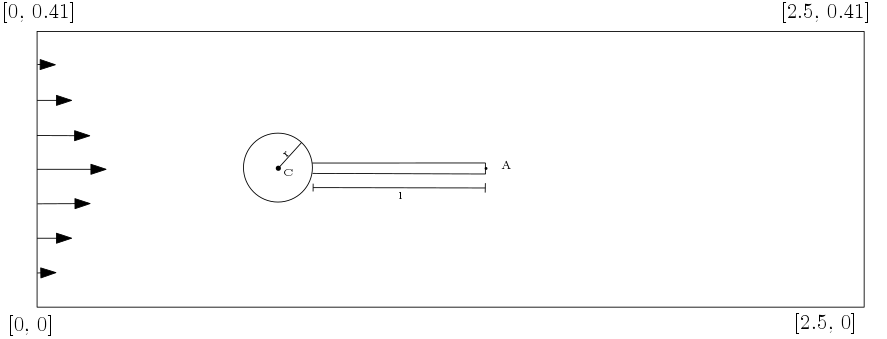
\includegraphics[scale=0.5]{./Fig/turekflag.png}
\end{figure}

Several quantites for comparion is presented in \cite{Hron2006} for validation purposes. We will report
\begin{itemize}
\item The position of point A(t) as the strucutre undergoes deformation.
\item Drag and lift forces exerted on of the whole interior geometry in contact with the fluid, consisting of the rigid circle and the elastic beam. 
\begin{align*}
(F_D, F_L) = \int_{\Gamma} \mathbf{\sigma} \cdot \mathbf{n} dS
\end{align*}
Where \textbf{n} is the unit normal vector, pointing into the fluid domain. 
\end{itemize}
The amplitude and mean values for the time dependent properties are calculated from the last period of oscillations, together with the period. 

\begin{table}[h]
\centering
\caption{Benchmark environment}
\label{my-label}
\begin{tabular}{ |p{3cm}||p{3cm}|p{3cm}|p{3cm}|  }
 \hline
 \multicolumn{4}{|c|}{Solid parameters} \\
 \hline
 parameter              & FSI1 & FSI2 & FSI3 \\
 \hline
 $\rho^s [10^{3} \frac{kg}{m^3}]$ & 1    & 10   & 1    \\
$\nu^s$ & 0.4  & 0.4  & 0.4  \\
$\mu^s  [10^{6}\frac{kg}{ms^2}]$  & 0.5  & 0.5  & 2.0  \\
 \hline
 \multicolumn{4}{|c|}{Fluid parameters} \\
 \hline
$\rho^f [10^{3}\frac{kg}{m^3}]$ & 1    & 1    & 1    \\
$\nu^f  [10^{-3}\frac{m^2}{s}]$  & 1    & 1    & 1    \\
U                      & 0.2  & 1    & 2    \\
parameter              & FSI1 & FSI2 & FSI3 \\
Re                     & 20   & 100  & 200 \\
\hline
\end{tabular}
\end{table}


\subsection{FSI1}
The first environment yields a steady state solution for the system. It is meant as a basic implementation test as it applies small deformations to the system. Therefore is provides a test for the solving procedure, but doesn't excess large constrain of choice of mesh extrapolation operator. 

\begin{table}[h!]
\centering
\caption{FSI 1}
\label{my-label}
\begin{tabular}{ |p{2.5cm}||p{1cm}|p{1cm}|p{2.3cm}|p{2.3cm}|p{1.2cm}|p{1.2cm}|}
 \hline
  \multicolumn{7}{|c|}{$\Delta t = 0.5$} \\
   \hline
 Model & nel & ndof & ux of A [x $10^{3}$]  &uy of A [x $10^{3}$]& Drag  & Lift \\
 \hline
Biharmonic bc2 & 1 &1 & 0.0228  &  0.7740  & 14.17280  &  0.7614 \\
 \hline
Biharmonic bc1 & 1 &1 & 0.0228 &   0.7737  & 14.17281 &  0.7612  \\
 \hline
Elastic        & 1 &1 & 0.0227  &  0.7960  & 14.17283 &  0.7607  \\
 \hline
Laplace        & 1 &1 & 0.0227  &  0.7958  & 14.17285 &  0.7607   \\
 \hline
  \multicolumn{7}{|c|}{$\Delta t = 0.1$} \\
   \hline
 Model & nel & ndof & ux of A [x $10^{3}$]  &uy of A [x $10^{3}$]& Drag  & Lift \\
 \hline
Biharmonic bc2 & 1 &1 & 0.0228 &  0.7743  & 14.17279 & 0.76162  \\
 \hline
Biharmonic bc1 & 1 &1 & 0.0228  &  0.7739 & 14.17280 & 0.76142 \\
 \hline
Elastic       & 1 &1 & 0.0228  &  0.7962  & 14.17281 & 0.76092 \\
 \hline
Laplace        & 1 &1 & 0.0228  & 0.7961  & 14.17284 & 0.76090 \\
\hline
\end{tabular}
\end{table}

\subsection{FSI2}
The second environment results in a periodic solution. It proved to be one of the most demanding tests due to its large deformation, leading to the risk of entangled mesh cells. As such this raised the need for a high quality extrapolation of the solid deformation.
\\
\subsection{FSI3}    
The final environment does not induce deformation to the extent of the FSI2 benchmark. However a critical phase in the transition to the periodic solution was discovered, where the pressure oscillation induces a large deformation to the system. 

\begin{table}[h!]
\centering
\caption{FSI 3}
\label{my-label}
\begin{tabular}{lllll}
 \hline
Test & x-comp A          & y-comp A             & drag                   & lift                 \\
 \hline
bc1 &                   &                      & 442.9 +/ 17.26         & 2.83 +- 148.8        \\
 \hline
bc2 &                   &                      & 442.8 +/ 17.44         & 3.06 +-147.9         \\
 \hline
Ref & 2.69  2.53  &   1.48  34.38 5.3   & 457. 22.66 10.9 & 2.22 149.78 5.3 \\
 \hline
\end{tabular}
\end{table}


\section{Mesh movement}
The final enviroment 
%\newpage

%\chapter{Conclusion and further research}

In this thesis, a monolithic fluid-structure interaction solver in an arbitrary Lagrangian Eulerian description have been presented. This inline with the original goal of this thesis. However, verification of code was not achieved, however successful validation through the benchmark presented in~\cite{Hron2006} indicates the code still represents the mathematical model correctly enough. Thus it opens up the possibility that the verification of code test it self might have been erroneous. \\

An investigation of long term temporal stability of the FSI benchmark showed the implicit Crank-Nicolson was not applicable for time steps $\Delta t > 0.001$. To overcome the stability issues, a shifted Crank-Nicolson scheme was introduced, were long time temporal stability was obtained for $\Delta t \leq 0.01$. Software profiling motivated run-time optimizations of the Newton solver, where a combination of Jacobian reuse and lower-order polynomials to assemble the Jacobian matrix proved most beneficial in terms of computational efficiency. \\

In order to further explore all aspects of the FSI problem, I have also compared three different mesh lifting operators, focusing on mesh regularity and computational efficiency. The Laplace lifting operator proved to be the most efficient method, while the biharmonic operator was the most rigorous, however at the cost of computational cost. The linear elastic model failed for all tests expect the FSI-1 problem, meaning it was only valid for small deformations. 

\newpage
\subsection*{Future research}
To pursue a successful verification of code is the primary future goal, which is necessary remove any doubt that the mathematical model is solved correctly. In addition, several extensions are possible. Several publications have showed the linear elastic lifiting operator applicable for a wide range of FSI problems. Therefore, further investigation is planned to investigate why the operator did not perform in my work. \\

Hoping to extend into 3D simulations, an implementation of iterative Krylov methods by block preconditioning are necessary, to overcome the CPU demanding nature of the monolithic FSI formulation. A substantial amount of time during the work of this thesis have been put into trying to implement the partitioned algorithm presented in \cite{Fernandez2007}. In the end, I was not able to finalize this project, but future research will be spent on finding the last mistakes. A projection method would allow for a wider variety of fluid schemes, making the whole fluid equation linear. Thus, having the potential of further speeding up the solution process.



\bibliographystyle{plain}
\bibliography{./Cite/Books,./Cite/ALECoupled,./Cite/Decoupled,./Cite/NavierStokes,./Cite/Verification,./Cite/EulerianFormulation,./Cite/Meshupdate}
\end{document}  
